\documentclass[11pt,preprint]{elsarticle}

\usepackage{lmodern}
%%%% My spacing
\usepackage{setspace}
\setstretch{1.2}
\DeclareMathSizes{12}{14}{10}{10}

% Wrap around which gives all figures included the [H] command, or places it "here". This can be tedious to code in Rmarkdown.
\usepackage{float}
\let\origfigure\figure
\let\endorigfigure\endfigure
\renewenvironment{figure}[1][2] {
    \expandafter\origfigure\expandafter[H]
} {
    \endorigfigure
}

\let\origtable\table
\let\endorigtable\endtable
\renewenvironment{table}[1][2] {
    \expandafter\origtable\expandafter[H]
} {
    \endorigtable
}


\usepackage{ifxetex,ifluatex}
\usepackage{fixltx2e} % provides \textsubscript
\ifnum 0\ifxetex 1\fi\ifluatex 1\fi=0 % if pdftex
  \usepackage[T1]{fontenc}
  \usepackage[utf8]{inputenc}
\else % if luatex or xelatex
  \ifxetex
    \usepackage{mathspec}
    \usepackage{xltxtra,xunicode}
  \else
    \usepackage{fontspec}
  \fi
  \defaultfontfeatures{Mapping=tex-text,Scale=MatchLowercase}
  \newcommand{\euro}{€}
\fi

\usepackage{amssymb, amsmath, amsthm, amsfonts}

\def\bibsection{\section*{References}} %%% Make "References" appear before bibliography


\usepackage[numbers]{natbib}

\usepackage{longtable}
\usepackage[margin=2.3cm,bottom=2cm,top=2.5cm, includefoot]{geometry}
\usepackage{fancyhdr}
\usepackage[bottom, hang, flushmargin]{footmisc}
\usepackage{graphicx}
\numberwithin{equation}{section}
\numberwithin{figure}{section}
\numberwithin{table}{section}
\setlength{\parindent}{0cm}
\setlength{\parskip}{1.3ex plus 0.5ex minus 0.3ex}
\usepackage{textcomp}
\renewcommand{\headrulewidth}{0.2pt}
\renewcommand{\footrulewidth}{0.3pt}

\usepackage{array}
\newcolumntype{x}[1]{>{\centering\arraybackslash\hspace{0pt}}p{#1}}

%%%%  Remove the "preprint submitted to" part. Don't worry about this either, it just looks better without it:
\makeatletter
\def\ps@pprintTitle{%
  \let\@oddhead\@empty
  \let\@evenhead\@empty
  \let\@oddfoot\@empty
  \let\@evenfoot\@oddfoot
}
\makeatother

 \def\tightlist{} % This allows for subbullets!

\usepackage{hyperref}
\hypersetup{breaklinks=true,
            bookmarks=true,
            colorlinks=true,
            citecolor=blue,
            urlcolor=blue,
            linkcolor=blue,
            pdfborder={0 0 0}}


% The following packages allow huxtable to work:
\usepackage{siunitx}
\usepackage{multirow}
\usepackage{hhline}
\usepackage{calc}
\usepackage{tabularx}
\usepackage{booktabs}
\usepackage{caption}


\newenvironment{columns}[1][]{}{}

\newenvironment{column}[1]{\begin{minipage}{#1}\ignorespaces}{%
\end{minipage}
\ifhmode\unskip\fi
\aftergroup\useignorespacesandallpars}

\def\useignorespacesandallpars#1\ignorespaces\fi{%
#1\fi\ignorespacesandallpars}

\makeatletter
\def\ignorespacesandallpars{%
  \@ifnextchar\par
    {\expandafter\ignorespacesandallpars\@gobble}%
    {}%
}
\makeatother


% definitions for citeproc citations
\NewDocumentCommand\citeproctext{}{}
\NewDocumentCommand\citeproc{mm}{%
\href{\#cite.\detokenize{#1}}{#2}\nocite{#1}}

\makeatletter
% allow citations to break across lines
\let\@cite@ofmt\@firstofone
% avoid brackets around text for \cite:
\def\@biblabel#1{}
\def\@cite#1#2{{#1\if@tempswa , #2\fi}}
\makeatother
\newlength{\cslhangindent}
\setlength{\cslhangindent}{1.5em}
\newlength{\csllabelwidth}
\setlength{\csllabelwidth}{3em}
\newenvironment{CSLReferences}[2] % #1 hanging-indent, #2 entry-spacing
{\begin{list}{}{%
	\setlength{\itemindent}{0pt}
	\setlength{\leftmargin}{0pt}
	\setlength{\parsep}{0pt}
	% turn on hanging indent if param 1 is 1
	\ifodd #1
	\setlength{\leftmargin}{\cslhangindent}
	\setlength{\itemindent}{-1\cslhangindent}
	\fi
	% set entry spacing
	\setlength{\itemsep}{#2\baselineskip}}}
{\end{list}}

\usepackage{calc}
\newcommand{\CSLBlock}[1]{\hfill\break\parbox[t]{\linewidth}{\strut\ignorespaces#1\strut}}
\newcommand{\CSLLeftMargin}[1]{\parbox[t]{\csllabelwidth}{\strut#1\strut}}
\newcommand{\CSLRightInline}[1]{\parbox[t]{\linewidth - \csllabelwidth}{\strut#1\strut}}
\newcommand{\CSLIndent}[1]{\hspace{\cslhangindent}#1}


\urlstyle{same}  % don't use monospace font for urls
\setlength{\parindent}{0pt}
\setlength{\parskip}{6pt plus 2pt minus 1pt}
\setlength{\emergencystretch}{3em}  % prevent overfull lines
\setcounter{secnumdepth}{5}

%%% Use protect on footnotes to avoid problems with footnotes in titles
\let\rmarkdownfootnote\footnote%
\def\footnote{\protect\rmarkdownfootnote}
\IfFileExists{upquote.sty}{\usepackage{upquote}}{}

%%% Include extra packages specified by user

%%% Hard setting column skips for reports - this ensures greater consistency and control over the length settings in the document.
%% page layout
%% paragraphs
\setlength{\baselineskip}{12pt plus 0pt minus 0pt}
\setlength{\parskip}{12pt plus 0pt minus 0pt}
\setlength{\parindent}{0pt plus 0pt minus 0pt}
%% floats
\setlength{\floatsep}{12pt plus 0 pt minus 0pt}
\setlength{\textfloatsep}{20pt plus 0pt minus 0pt}
\setlength{\intextsep}{14pt plus 0pt minus 0pt}
\setlength{\dbltextfloatsep}{20pt plus 0pt minus 0pt}
\setlength{\dblfloatsep}{14pt plus 0pt minus 0pt}
%% maths
\setlength{\abovedisplayskip}{12pt plus 0pt minus 0pt}
\setlength{\belowdisplayskip}{12pt plus 0pt minus 0pt}
%% lists
\setlength{\topsep}{10pt plus 0pt minus 0pt}
\setlength{\partopsep}{3pt plus 0pt minus 0pt}
\setlength{\itemsep}{5pt plus 0pt minus 0pt}
\setlength{\labelsep}{8mm plus 0mm minus 0mm}
\setlength{\parsep}{\the\parskip}
\setlength{\listparindent}{\the\parindent}
%% verbatim
\setlength{\fboxsep}{5pt plus 0pt minus 0pt}



\begin{document}



\begin{frontmatter}  %

\title{Exploring Risk and Uncertainty}

% Set to FALSE if wanting to remove title (for submission)




\author[Add1]{Sihlelelwe Nzima}
\ead{}





\address[Add1]{Stellenbosch University, Stellenbosch, South Africa}


\begin{abstract}
\small{
This note examines whether volatility on the local equity market has
increased, how it relates to offshore economic and policy uncertainty,
and what this means for building risk ballasts into local equity funds.
Local volatility has become more episodic since 2020 rather than
permanently higher, and its spikes are largely imported: global implied
volatility and oil price volatility explain close to three quarters of
the monthly variation in Capped SWIX volatility, while local currency
volatility adds little. The SafeCore fund has outperformed its benchmark
but has not been a risk ballast: its volatility matches the market's,
two gold miners carry almost half of its risk, and its quality-momentum
style has no low-volatility tilt. The opportunity for stock selection,
measured by dispersion and correlation, was weak from 2022 to 2024 but
has improved since 2025, and rising bond and currency volatility have
tended to precede less rewarding conditions for stock pickers.
}
\end{abstract}

\vspace{1cm}


\begin{keyword}
\footnotesize{
Volatility \sep GARCH \sep Policy uncertainty \sep Factor exposure
\sep Dispersion \\
\vspace{0.3cm}
}
\footnotesize{
\textit{JEL classification} G11 \sep G15 \sep C58
}
\end{keyword}



\vspace{0.5cm}

\end{frontmatter}

\setcounter{footnote}{0}



%________________________
% Header and Footers
%%%%%%%%%%%%%%%%%%%%%%%%%%%%%%%%%
\pagestyle{fancy}
\chead{}
\rhead{}
\lfoot{}
\rfoot{\footnotesize Page \thepage}
\lhead{}
%\rfoot{\footnotesize Page \thepage } % "e.g. Page 2"
\cfoot{}

%\setlength\headheight{30pt}
%%%%%%%%%%%%%%%%%%%%%%%%%%%%%%%%%
%________________________

\headsep 35pt % So that header does not go over title




\section{\texorpdfstring{Introduction
\label{Introduction}}{Introduction }}\label{introduction}

A recent seminar argued that oil price volatility and global policy
uncertainty are spilling over into local equity markets, and that local
portfolios should lean more towards lower-volatility stocks. This note
tests that argument in three steps. Part A establishes whether local
volatility has increased and whether it mirrors the global experience.
Part B evaluates how the SafeCore fund has navigated volatility and what
its factor exposures are. Part C studies dispersion and correlation, to
gauge the alpha opportunity in the market since 2020.

\section{\texorpdfstring{Part A: Has local volatility increased?
\label{PartA}}{Part A: Has local volatility increased? }}\label{part-a-has-local-volatility-increased}

\subsection{Data}\label{data}

Local index returns (Capped SWIX, Top 40, Mid Caps and Small Caps, in
rand) are available from January 2015, so the analysis runs from January
2015 to September 2026. The global comparison uses total return indexes
in US dollars: MSCI ACWI, MSCI Emerging Markets, the S\&P 500, the Euro
Stoxx 50 and the Nikkei 225. To link volatility to uncertainty, the
analysis uses implied volatility (VIX, V2X, VXEEM), economic policy
uncertainty (EPU) indexes, US bond market volatility (MOVE), Brent oil
volatility and currency volatility (SAVI for USDZAR and JP Morgan's
global FX volatility index).

Two data issues were treated. The global and European EPU indexes are
monthly values repeated on every day, so all comparisons with them are
done at a monthly frequency. The SAVI index is quoted as a decimal
rather than a percentage on 109 days (mostly March to June 2021); these
values were rescaled.

\subsection{Realised volatility}\label{realised-volatility}

Figure \ref{rollvol} plots the rolling three-month realised volatility
of each index, with every other index shown in grey for context. The
shaded bands mark five market events: two South African political shocks
(Nenegate in December 2015, and the March 2017 cabinet reshuffle
followed by the sovereign downgrade to junk) and three global shocks
(the COVID-19 crash, the 2022 Ukraine war and oil price shock, and the
April 2025 US tariff shock). The COVID-19 crash dominates every series,
with local volatility peaking above 50\%. Outside of 2020, local
volatility has been punctuated by shorter spikes, most of which coincide
with the global events.

\begin{figure}[H]

{\centering 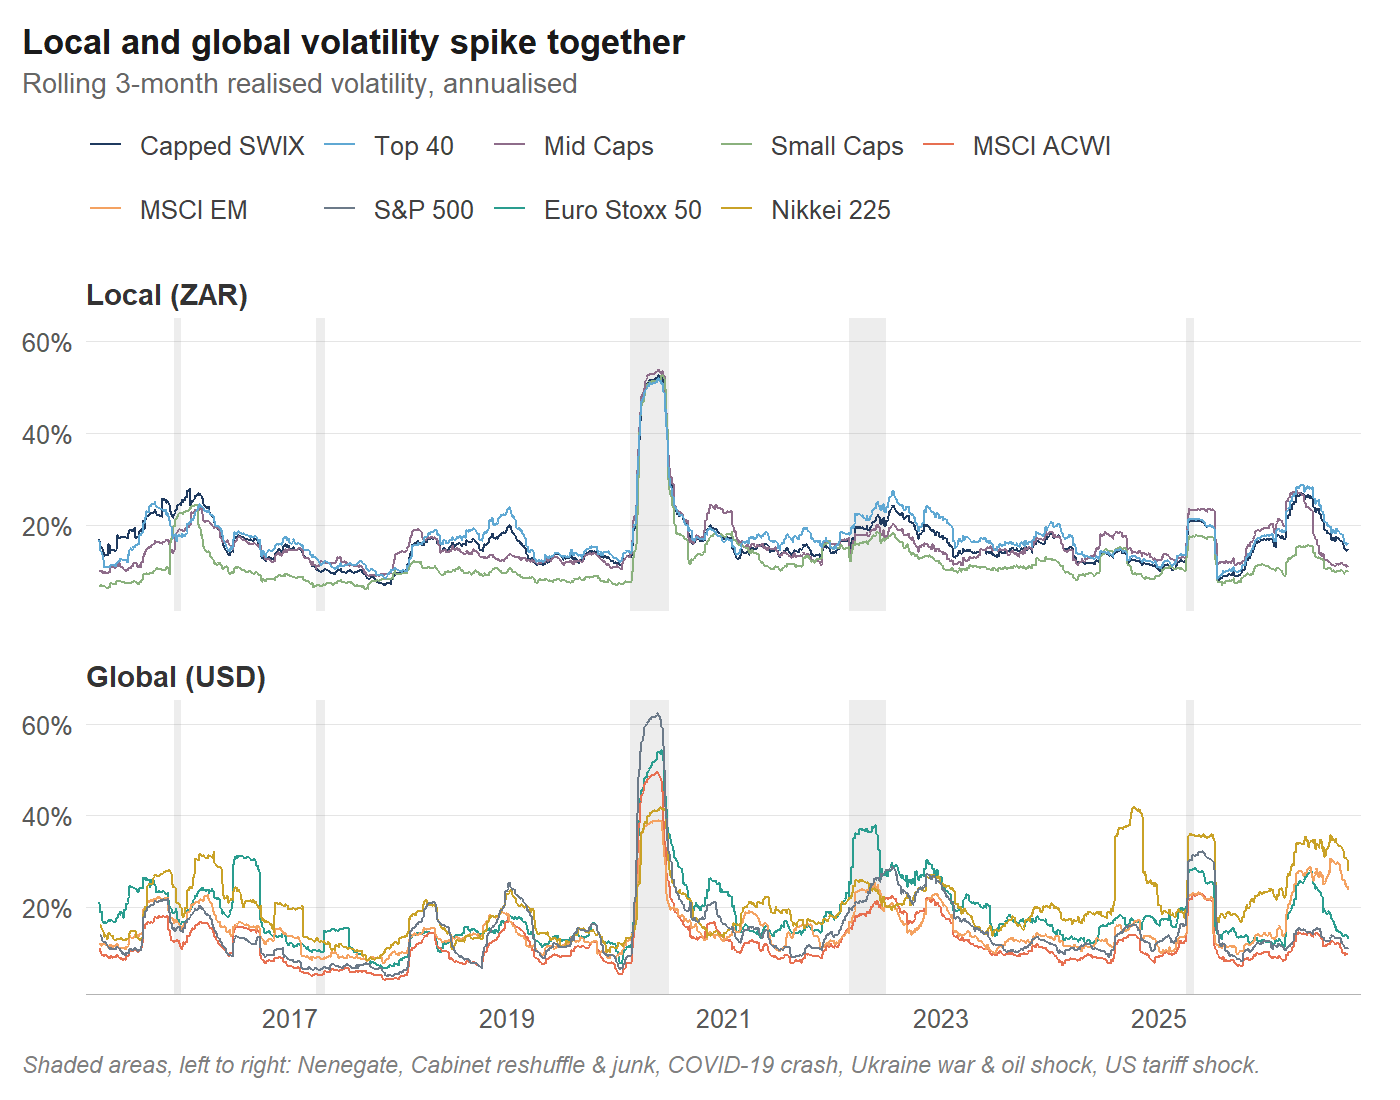
\includegraphics[width=1\linewidth]{Question1_files/figure-latex/rollvol-1} 

}

\caption{Rolling 3-month realised volatility: each panel highlights one index against all others (grey) \label{rollvol}}\label{fig:rollvol}
\end{figure}

Figure \ref{calvol} shows the same story by calendar year. The notable
recent feature is 2026: Capped SWIX volatility (about 21\% year-to-date)
is well above that of developed markets (MSCI ACWI about 12\%) and much
closer to emerging markets (MSCI EM about 25\%). Local volatility in
2025-26 is therefore tracking the emerging market experience rather than
the developed market one.

\begin{figure}[H]

{\centering 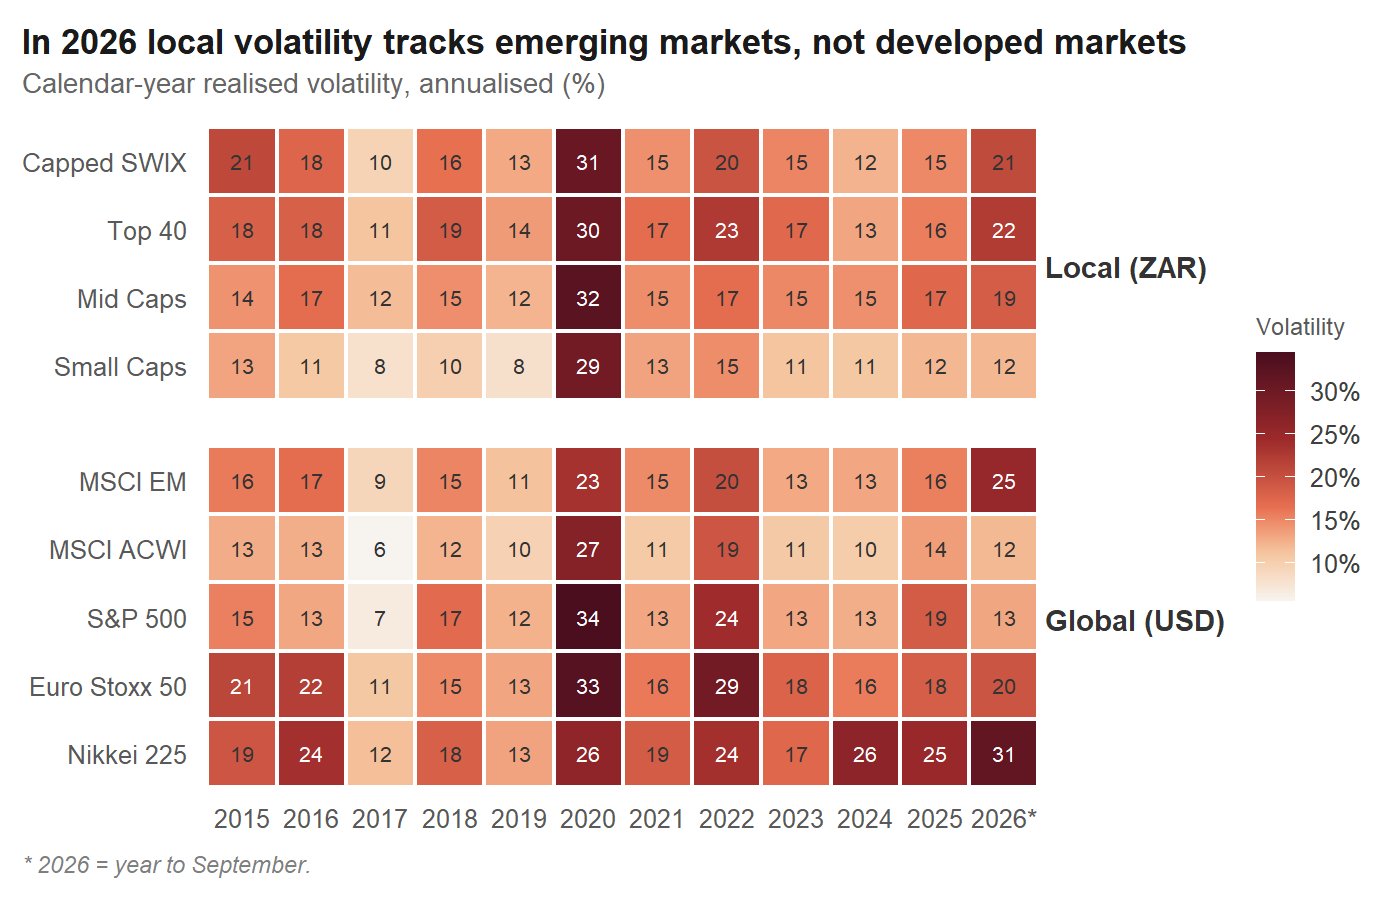
\includegraphics[width=1\linewidth]{Question1_files/figure-latex/calvol-1} 

}

\caption{Calendar-year realised volatility (\%) \label{calvol}}\label{fig:calvol}
\end{figure}

Figure \ref{regime} compares average volatility before and after 2020,
and the share of days each index spends in a high-volatility state
(above its own long-run 80th percentile). Including the COVID period,
every index shows higher volatility after 2020. Once the COVID crash is
excluded, however, average Capped SWIX volatility barely rises (from
15.4\% to 16.0\%), while the share of high-volatility days still
increases (from 17\% to 22\%). The increase in local volatility is
therefore better described as \textbf{more frequent volatility episodes}
than as a permanently higher level. It is also smaller than the increase
seen in developed markets such as the S\&P 500 and the Nikkei.

\begin{figure}[H]

{\centering 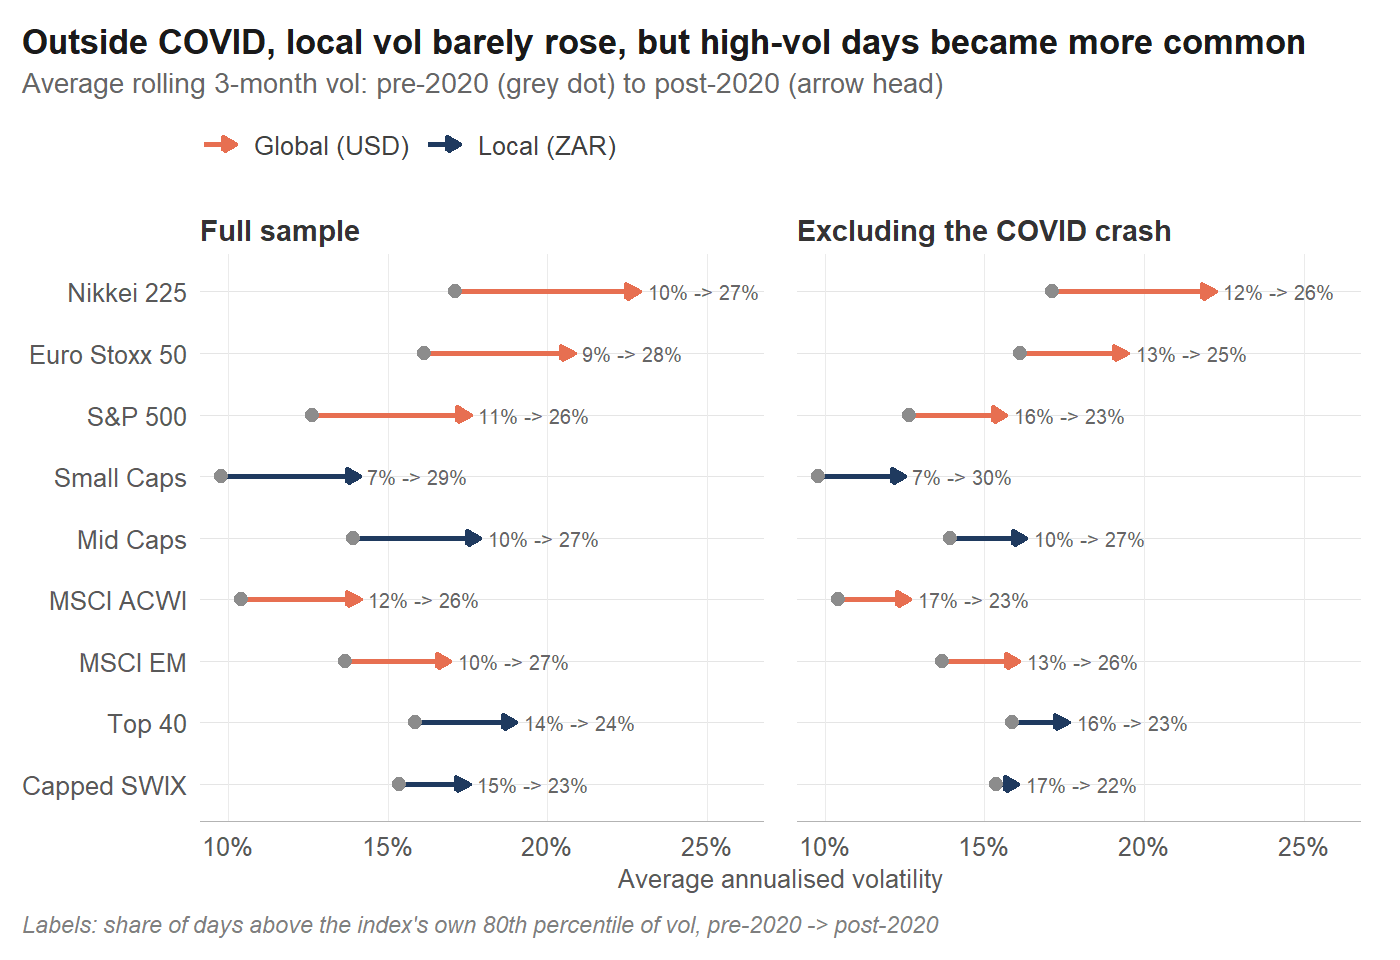
\includegraphics[width=1\linewidth]{Question1_files/figure-latex/regime-1} 

}

\caption{Average rolling volatility and share of high-volatility days, before and after 2020 \label{regime}}\label{fig:regime}
\end{figure}

\subsection{Home-grown or imported
volatility?}\label{home-grown-or-imported-volatility}

Figure \ref{events} measures how far rolling volatility rose around each
event, from the level just before the event to its peak during the event
and the following month. The two local political shocks were
short-lived: Nenegate lifted local volatility by about 6 percentage
points, roughly three times the global move, but the 2017 reshuffle and
junk downgrade barely moved local volatility at all, suggesting the
downgrade was largely priced in. The three global shocks, by contrast,
lifted local volatility by about as much as global volatility (roughly 8
to 9 points in 2022 and 2025, and close to 40 points during COVID-19).
The large volatility episodes in the local market have therefore been
imported, while home-grown political shocks have been smaller and faded
quickly.

\begin{figure}[H]

{\centering 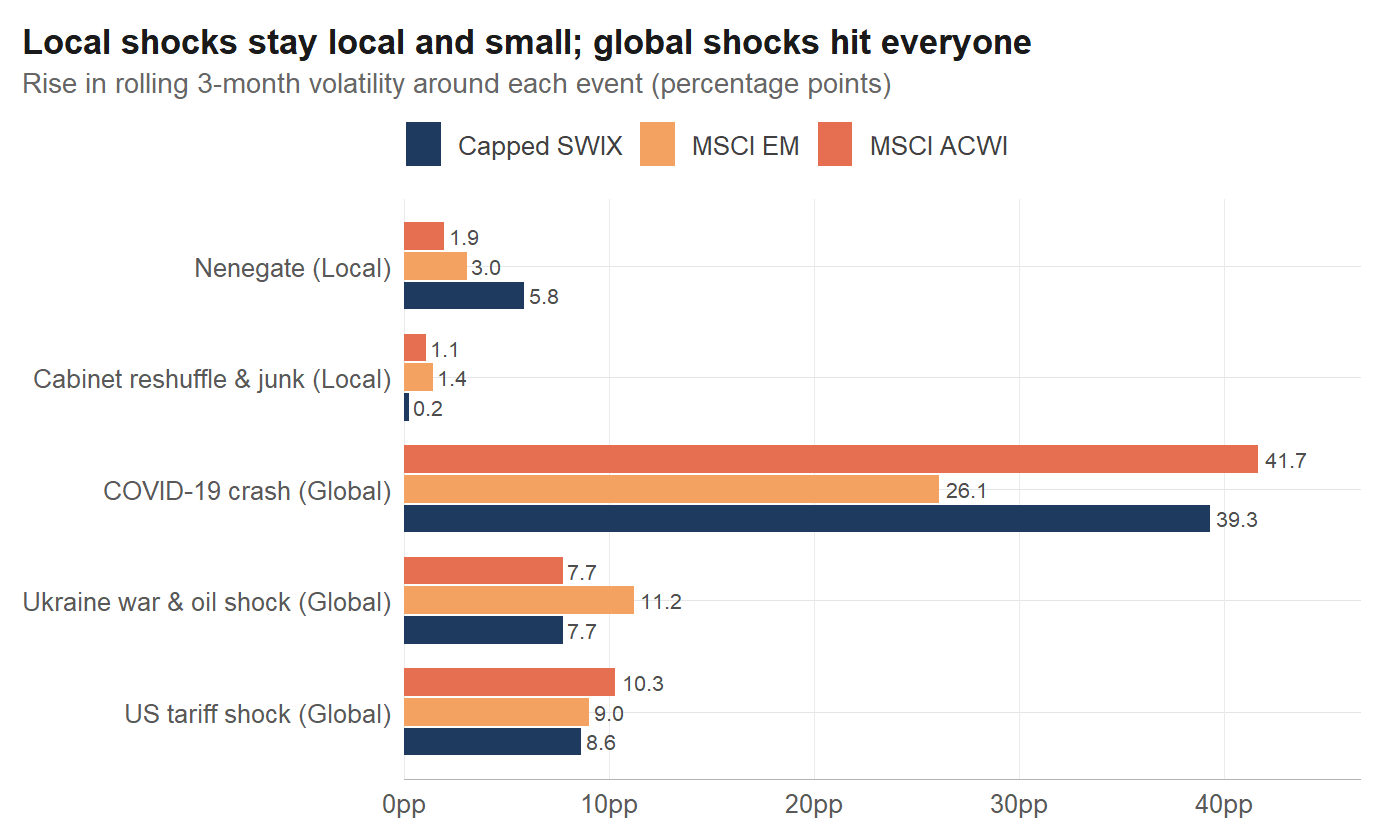
\includegraphics[width=1\linewidth]{Question1_files/figure-latex/events-1} 

}

\caption{Rise in rolling 3-month volatility around each event \label{events}}\label{fig:events}
\end{figure}

\subsection{Does local mirror global?}\label{does-local-mirror-global}

Figure \ref{rollcor} shows rolling one-year correlations between weekly
Capped SWIX returns and the global indexes. Weekly returns are used
because the JSE closes before US markets open, which biases daily
correlations downward. The correlation with MSCI ACWI averages around
0.68 and rose to roughly 0.9 during the COVID crisis: in a global
sell-off, local and global markets move together, exactly when
diversification is needed most. More recently the correlation with
emerging markets has fallen, suggesting that part of the 2026 volatility
is local or EM-specific.

\begin{figure}[H]

{\centering 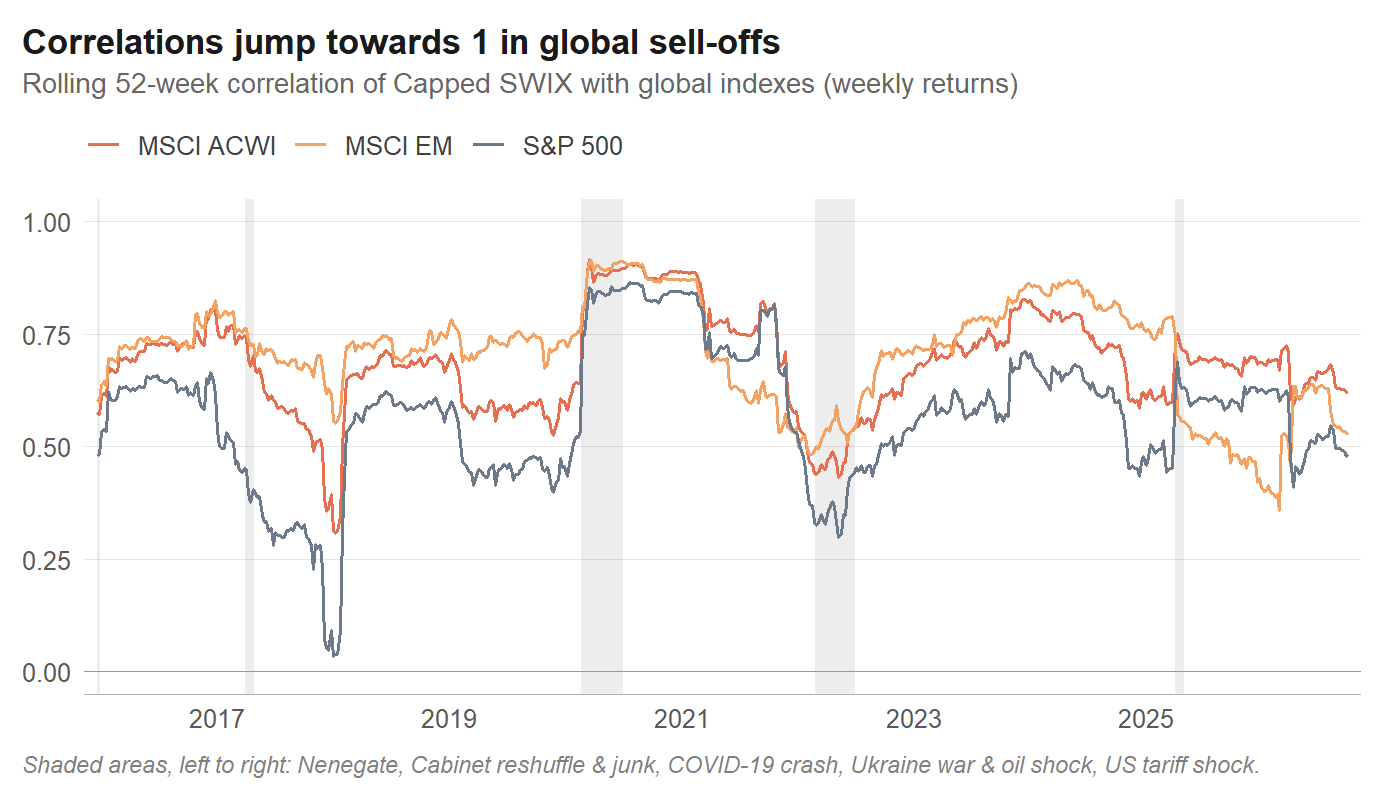
\includegraphics[width=1\linewidth]{Question1_files/figure-latex/rollcor-1} 

}

\caption{Rolling 52-week correlation of Capped SWIX with global indexes (weekly returns) \label{rollcor}}\label{fig:rollcor}
\end{figure}

\subsection{Conditional volatility}\label{conditional-volatility}

Ljung-Box tests on squared returns strongly reject the null of no ARCH
effects for all three series (p-values close to zero), confirming
volatility clustering. Comparing information criteria, the asymmetric
GARCH models fit better than the standard GARCH, so a GJR-GARCH(1,1) is
used with an AR(1) mean and skewed-t errors. Table \ref{tab:garch}
reports the key parameters and Ljung-Box tests on the standardised
residuals: the squared standardised residuals show no remaining
clustering (p-values of 0.71-0.99), confirming that the model captures
the volatility dynamics. Two results stand out. First, the symmetric
shock parameter (\(\alpha\)) is close to zero while the leverage
parameter (\(\gamma\)) is large: volatility rises after bad news but
hardly reacts to good news. Second, persistence is high (about 0.97
locally), implying a half-life of a volatility shock of roughly a month.
Local volatility shocks fade faster than global (MSCI ACWI) shocks but
slower than shocks to the broad EM index.

\begin{table}[H]
\centering
\caption{GJR-GARCH(1,1) parameters (AR(1) mean, skewed-t errors) and Ljung-Box (12 lags) p-values for the standardised residuals \label{tab:garch}} 
\begin{tabular}{lrrrrrrr}
  \toprule
Index & alpha & beta & gamma & Persistence & Half-life (days) & LB p (z) & LB p (z squared) \\ 
  \midrule
Capped SWIX & 0.002 & 0.903 & 0.132 & 0.969 & 21.970 & 0.047 & 0.987 \\ 
  MSCI ACWI & 0.000 & 0.865 & 0.232 & 0.976 & 28.316 & 0.447 & 0.713 \\ 
  MSCI EM & 0.013 & 0.848 & 0.181 & 0.949 & 13.277 & 0.620 & 0.801 \\ 
   \bottomrule
\end{tabular}
\end{table}

\begin{figure}[H]

{\centering 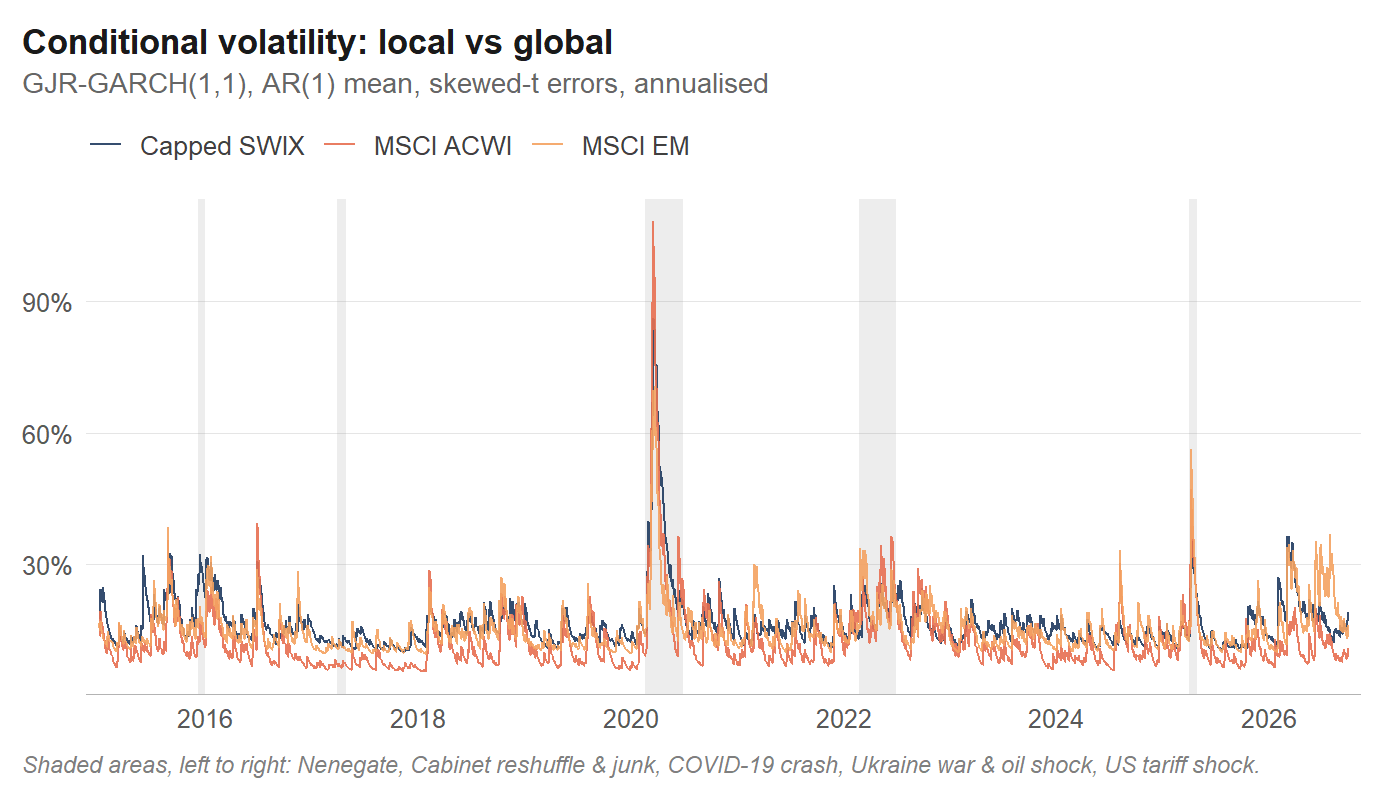
\includegraphics[width=1\linewidth]{Question1_files/figure-latex/sigma-1} 

}

\caption{GJR-GARCH conditional volatility, annualised \label{sigma}}\label{fig:sigma}
\end{figure}

\subsection{How much of local volatility is
imported?}\label{how-much-of-local-volatility-is-imported}

The rolling correlation above uses a fixed 52-week window. A DCC-GARCH
model (Engle, 2002) instead updates the correlations every week from the
latest shocks. It is fitted to weekly returns of the Capped SWIX, MSCI
ACWI and MSCI EM: each series has its own GJR-GARCH(1,1) with Student-t
errors, and a DCC(1,1) process with a multivariate t distribution models
the correlations of the standardised residuals. Table \ref{tab:dcc}
shows that the correlation dynamics are significant and persistent (a
half-life of about 16 weeks), while the asymmetric aDCC finds no
asymmetry (\(g\) = 0.00, likelihood-ratio p = 1.00): correlations
respond to the size of joint shocks, crash and rebound alike, rather
than only to joint falls.

Because the model gives the full conditional covariance matrix \(H_t\),
the share of local conditional variance explained by the two global
indexes can be computed every week, as
\(h_{lg,t}' H_{gg,t}^{-1} h_{lg,t} / h_{ll,t}\) (the R-squared of local
on global returns, using that week's covariances). Figure \ref{dcc}
colours local conditional volatility by this imported share. On average
about half (52\%) of local variance moves with global markets. The share
reaches two-thirds (65\%) in the COVID crash but falls to 46\% during
Nenegate, and it rises with the level of volatility: the bigger the
episode, the more of it is imported. The 2022 oil shock is an exception,
with only about half of local variance moving with global markets,
possibly because the resource-heavy local market reacted differently to
the commodity-price spike.

\begin{table}[H]
\centering
\caption{DCC and asymmetric DCC (aDCC) models of weekly Capped SWIX, MSCI ACWI and MSCI EM returns \label{tab:dcc}} 
\begin{tabular}{lrrrrrrr}
  \toprule
Model & a & b & g (asym.) & Half-life (wks) & Log-lik. & AIC & LR p-value \\ 
  \midrule
DCC & 0.020 & 0.938 &  & 16.091 & -3441.654 & 11.289 &  \\ 
  aDCC (asymmetric) & 0.020 & 0.938 & 0.000 & 16.090 & -3441.654 & 11.292 & 1.000 \\ 
   \bottomrule
\end{tabular}
\end{table}

\begin{figure}[H]

{\centering 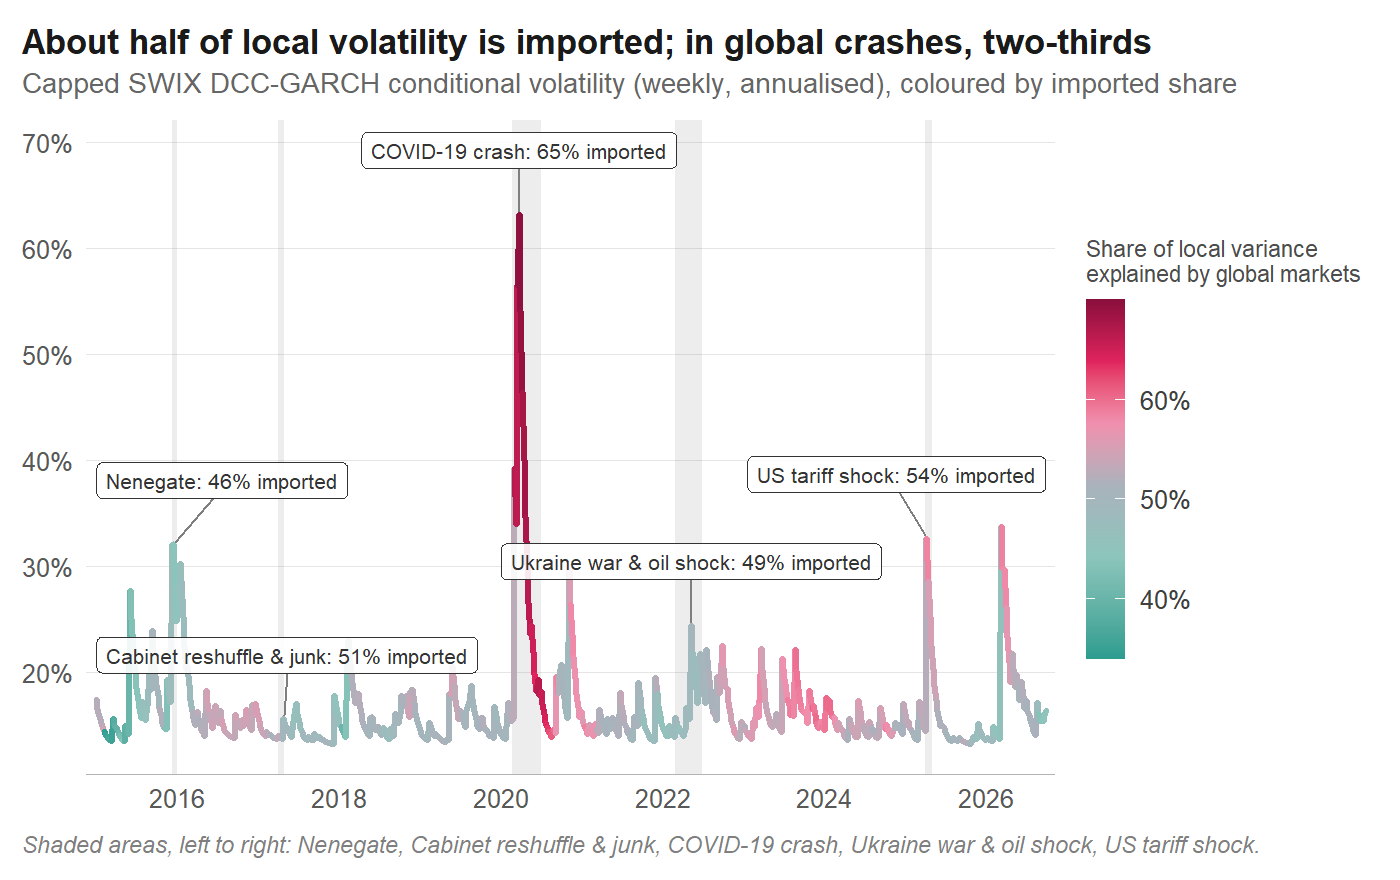
\includegraphics[width=1\linewidth]{Question1_files/figure-latex/dcc-1} 

}

\caption{Capped SWIX conditional volatility from the DCC model, coloured by the share of local variance explained by global markets \label{dcc}}\label{fig:dcc}
\end{figure}

\subsection{What drives local
volatility?}\label{what-drives-local-volatility}

Figure \ref{drivers} overlays monthly local GARCH volatility
(standardised) on each uncertainty measure, and Figure \ref{heat} maps
the strongest of their correlations as a network, in which the policy
uncertainty measures connect only to each other. Local volatility moves
closely with market-based measures of fear: global equity volatility
(correlation of 0.87 with MSCI ACWI volatility), implied volatility
(about 0.8 with VIX, V2X and VXEEM) and oil volatility (0.70). By
contrast, the news-based policy uncertainty indexes show almost no
correlation with local volatility (0.08 for global EPU). Policy
uncertainty appears to matter for markets only once it shows up as a
shock to global risk appetite or to oil prices.

\begin{figure}[H]

{\centering 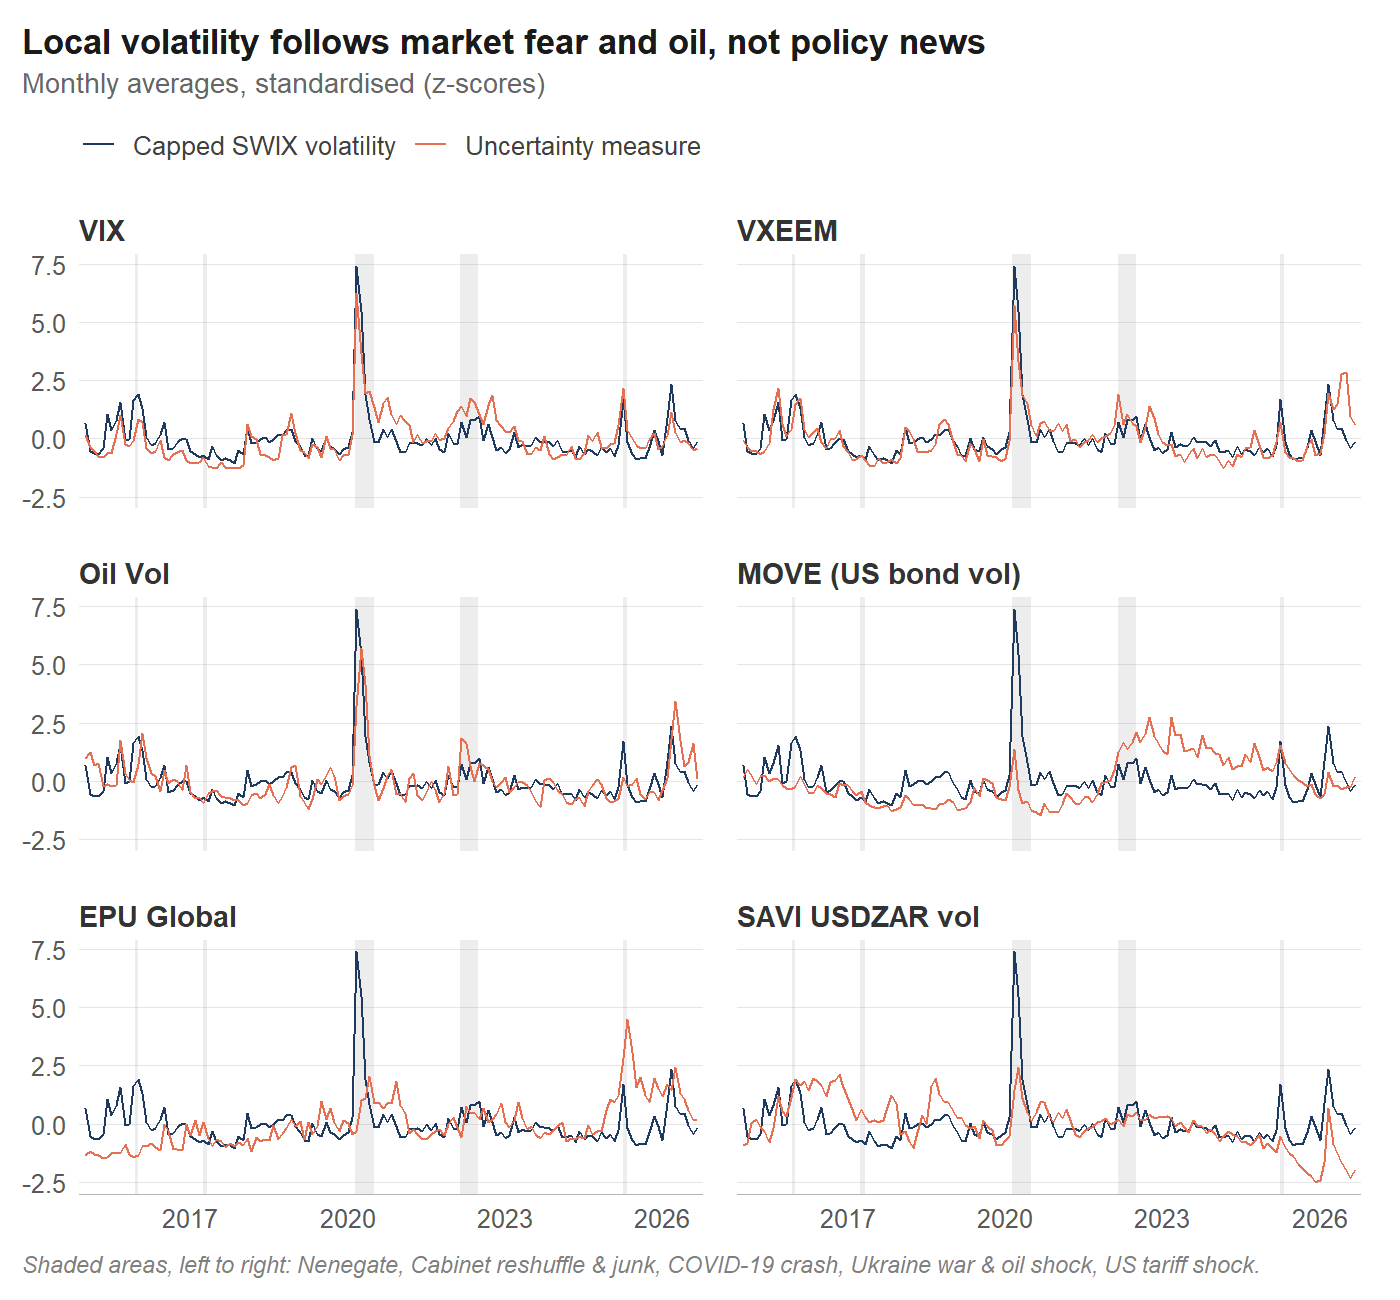
\includegraphics[width=1\linewidth]{Question1_files/figure-latex/drivers-1} 

}

\caption{Local volatility vs uncertainty measures (monthly, z-scores) \label{drivers}}\label{fig:drivers}
\end{figure}

\begin{figure}[H]

{\centering 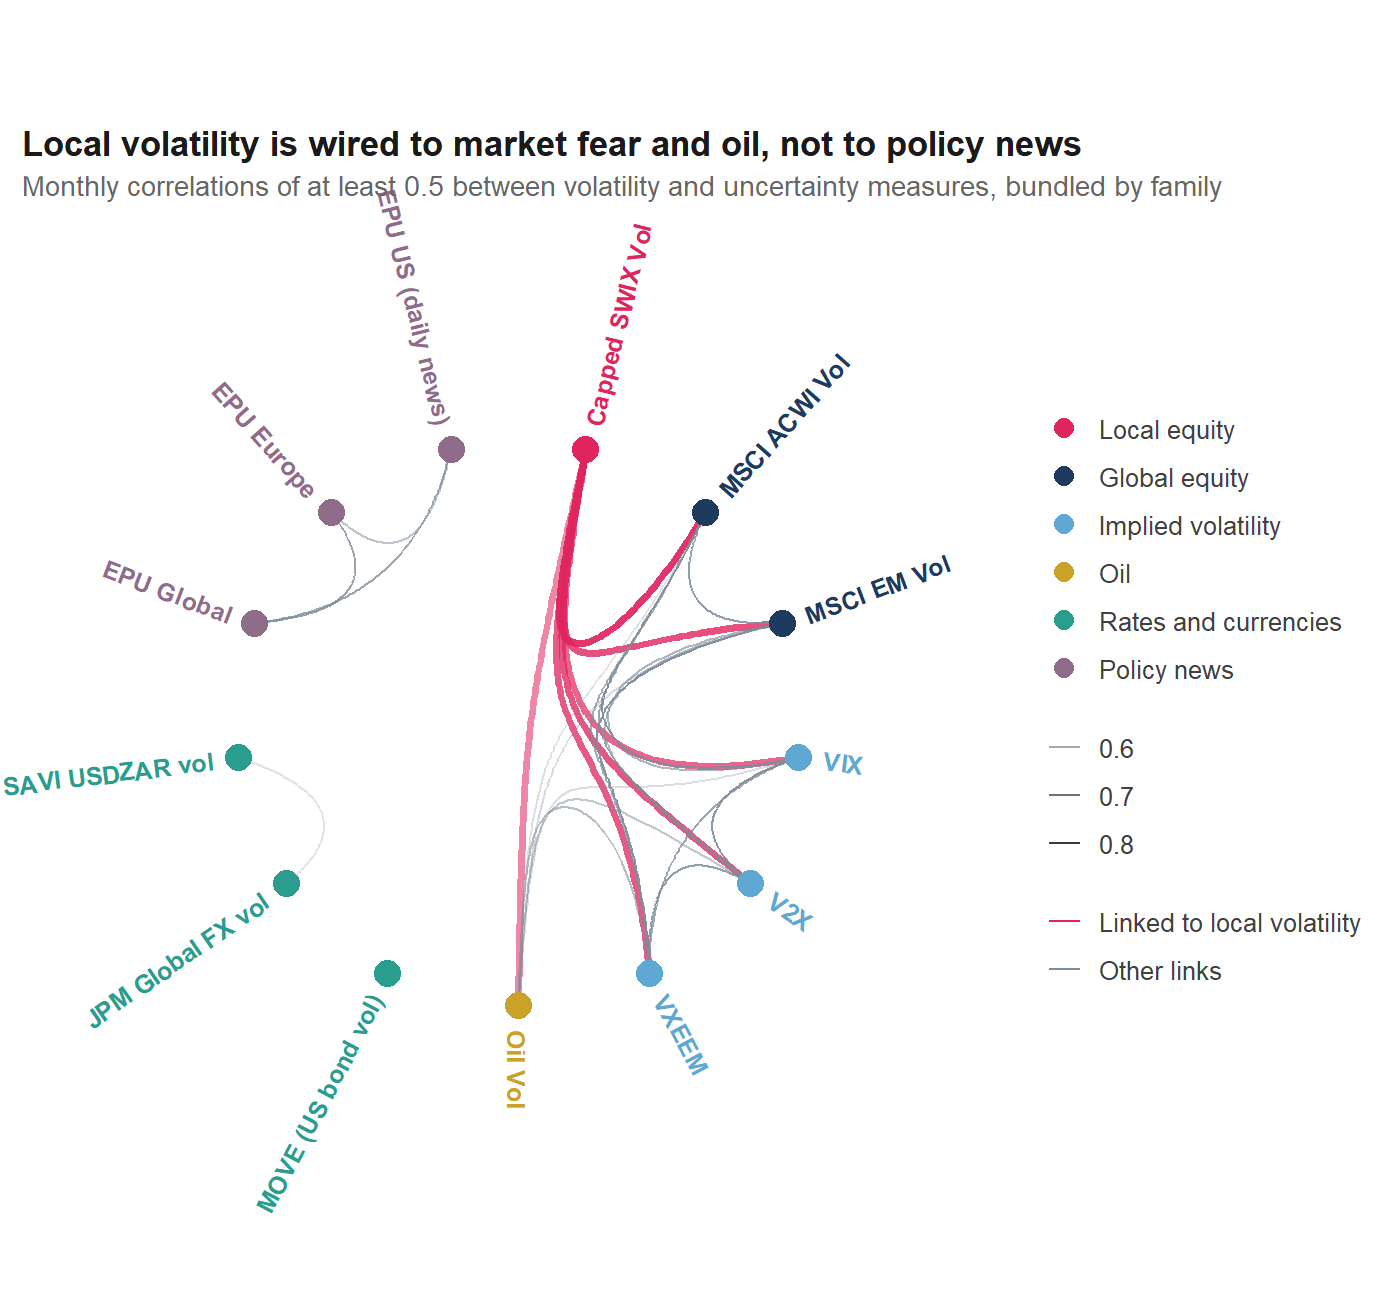
\includegraphics[width=1\linewidth]{Question1_files/figure-latex/heat-1} 

}

\caption{Correlation network of monthly volatility and uncertainty measures: curves join pairs with a correlation of at least 0.5, bundled by family \label{heat}}\label{fig:heat}
\end{figure}

Table \ref{tab:reg} formalises this with a regression of standardised
local volatility on the offshore measures. Standard errors are
Newey-West, because persistent monthly volatility series leave
autocorrelated residuals. The VIX and oil volatility are the dominant
and highly significant drivers, and the offshore measures alone explain
about 73\% of the monthly variation in local volatility. Adding local
currency volatility (SAVI) barely changes the fit and is not
significant. Global EPU enters negatively once the VIX is controlled
for, but it is only borderline significant (p = 0.04) and loses
significance when SAVI is added; as EPU and the VIX are correlated, this
coefficient should be read with caution.

\begin{table}[H]
\centering
\caption{Standardised regression of Capped SWIX GARCH volatility on uncertainty measures (monthly, Newey-West standard errors). R-squared: Offshore only = 0.73; Offshore + SAVI = 0.73 \label{tab:reg}} 
\begin{tabular}{llrrrr}
  \toprule
Model & Variable & Beta & Std. error & t-stat & p-value \\ 
  \midrule
Offshore only & VIX & 0.64 & 0.13 & 4.81 & 0.00 \\ 
  Offshore only & EPU Global & -0.19 & 0.09 & -2.07 & 0.04 \\ 
  Offshore only & MOVE US bond vol & -0.07 & 0.09 & -0.84 & 0.41 \\ 
  Offshore only & Oil Vol & 0.37 & 0.06 & 6.26 & 0.00 \\ 
  Offshore + SAVI & VIX & 0.62 & 0.13 & 4.72 & 0.00 \\ 
  Offshore + SAVI & EPU Global & -0.16 & 0.11 & -1.49 & 0.14 \\ 
  Offshore + SAVI & MOVE US bond vol & -0.06 & 0.09 & -0.73 & 0.47 \\ 
  Offshore + SAVI & Oil Vol & 0.37 & 0.07 & 5.49 & 0.00 \\ 
  Offshore + SAVI & SAVI USDZAR vol & 0.05 & 0.06 & 0.87 & 0.38 \\ 
   \bottomrule
\end{tabular}
\end{table}

\subsection{Implications for Part A}\label{implications-for-part-a}

Local volatility has not risen to a permanently higher level, but
volatility episodes have become more frequent since 2020, and in 2025-26
local volatility has tracked emerging markets rather than developed
markets. These episodes are largely imported: global risk-off shocks and
oil price volatility explain most of the variation, the share of local
variance that moves with global markets rises from about half in normal
times to two-thirds in a global crash, and volatility rises far more
after losses than after gains.

Was the seminar right that oil price volatility and global policy
uncertainty are spilling into local equities? Partly. Oil volatility
clearly feeds into local volatility, but policy uncertainty only seems
to matter once it turns into global market fear. For local equity funds,
the practical takeaway is that the risk worth protecting against is a
global sell-off rather than a rand shock, so any risk ballast
(lower-volatility stocks, rand-hedge exposure) should be judged on how
it holds up in those episodes. That is the lens used to evaluate
SafeCore in Part B.

Three caveats apply. The regressions capture associations rather than
causal effects. Monthly volatility measures are persistent, which is why
Newey-West standard errors are used; with about 140 monthly
observations, the borderline EPU result should still be read with
caution. Finally, local volatility is measured in rand and global
volatility in US dollars, so part of any gap between them, and part of
the imported share from the DCC model, reflects currency movements
rather than the equity markets themselves.

\section{\texorpdfstring{Part B: Does SafeCore navigate volatility?
\label{PartB}}{Part B: Does SafeCore navigate volatility? }}\label{part-b-does-safecore-navigate-volatility}

SafeCore is constructed without any explicit view on volatility, so the
question is whether it nonetheless behaves like a risk ballast, and if
not, why. The analysis first establishes \emph{whether} it navigates
volatility well, then \emph{where} its volatility comes from, and
finally \emph{what kind of fund} it is in terms of factor exposures. The
Capped SWIX (J433) is the benchmark throughout.

\subsection{Data and a ``risk ballast''
reference}\label{data-and-a-risk-ballast-reference}

SafeCore's daily returns are built from its month-end holdings and daily
stock returns from 2015, with weights rescaled to 100\% (at least 95\%
of the fund's weight has return data in every month) and allowed to
drift between rebalances. As a reference for what a low-volatility
strategy achieves, the Low Vol index is rebuilt from its constituents
with quarterly rebalancing (end of March, June, September and December),
which extends it from 2024 back to September 2020. Over 2024-2026, where
the two overlap, the rebuild has a daily correlation of 0.995 with the
actual index and a tracking error of 1.4\% a year, which is accurate
enough to use it for the earlier years.

\subsection{Performance through
volatility}\label{performance-through-volatility}

Table \ref{tab:score} summarises the trade-off. SafeCore has been a good
fund in return terms: since 2015 it returned 11.4\% a year against 8.7\%
for the benchmark, with an information ratio of about 0.5. But it has
not reduced risk. Its volatility equals the benchmark's, its beta is
close to one, and since 2020 its maximum drawdown was deeper than the
benchmark's. The rebuilt Low Vol index lowered volatility as intended,
but at a large cost in return over a strong market period, and without a
smaller drawdown.

\begin{table}[H]
\centering
\caption{Risk and return scorecard vs the Capped SWIX (returns, volatility, drawdown and tracking error in \%; Sharpe ratio uses STeFI as the risk-free rate) \label{tab:score}} 
\begin{tabular}{llrrrrrrr}
  \toprule
Period & Fund & Ann. return & Ann. vol & Sharpe & Max drawdown & Beta & Tracking error & Info. ratio \\ 
  \midrule
2015-2026 & Capped SWIX & 8.65 & 17.84 & 0.10 & -41.66 & 1.00 & 0.00 &  \\ 
  2015-2026 & SafeCore & 11.38 & 17.89 & 0.25 & -39.10 & 0.95 & 5.61 & 0.49 \\ 
  2015-2026 & Top 40 & 11.05 & 18.74 & 0.23 & -34.62 & 0.99 & 6.36 & 0.38 \\ 
  Sep 2020-2026 & Capped SWIX & 16.21 & 16.39 & 0.59 & -14.14 & 1.00 & 0.00 &  \\ 
  Sep 2020-2026 & Low Vol & 12.42 & 15.10 & 0.39 & -14.72 & 0.88 & 5.12 & -0.74 \\ 
  Sep 2020-2026 & SafeCore & 17.61 & 16.90 & 0.65 & -18.49 & 1.00 & 3.94 & 0.36 \\ 
  Sep 2020-2026 & Top 40 & 16.08 & 18.06 & 0.53 & -17.23 & 1.06 & 4.95 & -0.03 \\ 
   \bottomrule
\end{tabular}
\end{table}

Figure \ref{growth} shows where the outperformance came from and what it
did not change: SafeCore pulled ahead in 2016-2018 and again from 2020
(since when it has tracked the Top 40 closely), but in every major
sell-off it fell about as far as the market. Figure \ref{volratio} makes
the point directly: SafeCore was less volatile than the benchmark in
only about a quarter of rolling one-year windows, and has been slightly
more volatile since 2021. The Low Vol index was smoother in every
window, by about 8\% on average.

\begin{figure}[H]

{\centering 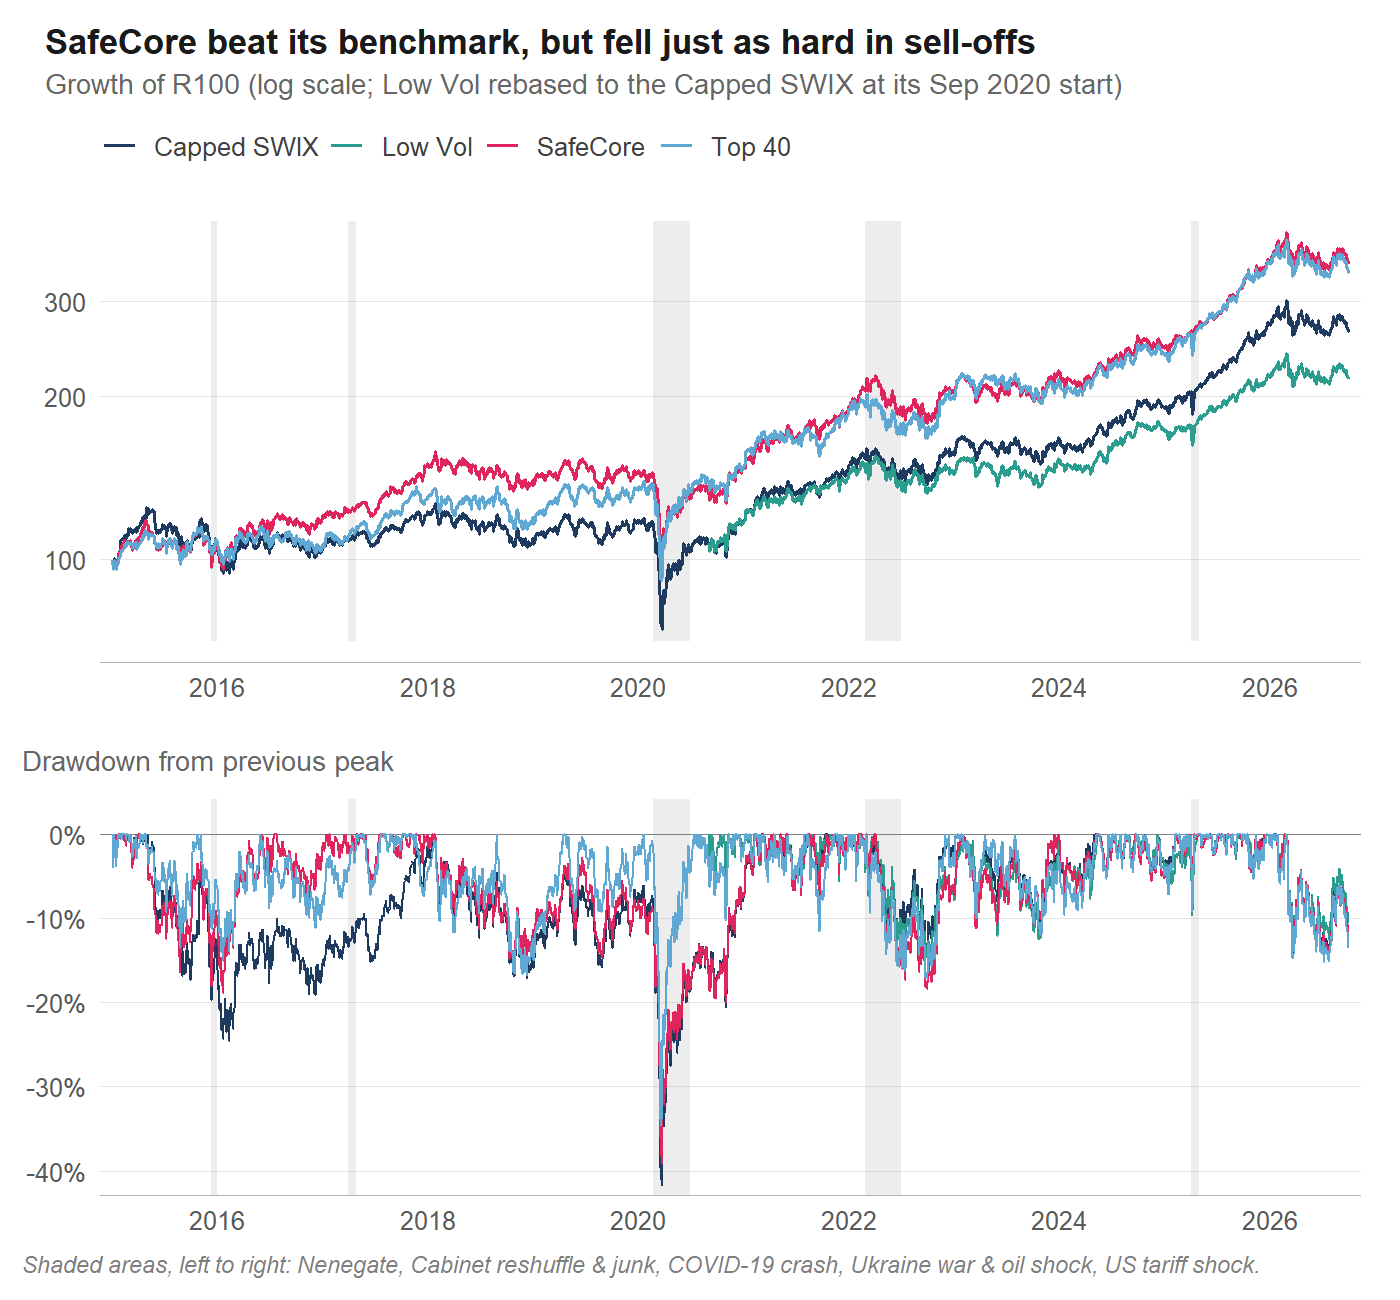
\includegraphics[width=1\linewidth]{Question1_files/figure-latex/growth-1} 

}

\caption{Growth of R100 and drawdowns \label{growth}}\label{fig:growth}
\end{figure}

\begin{figure}[H]

{\centering 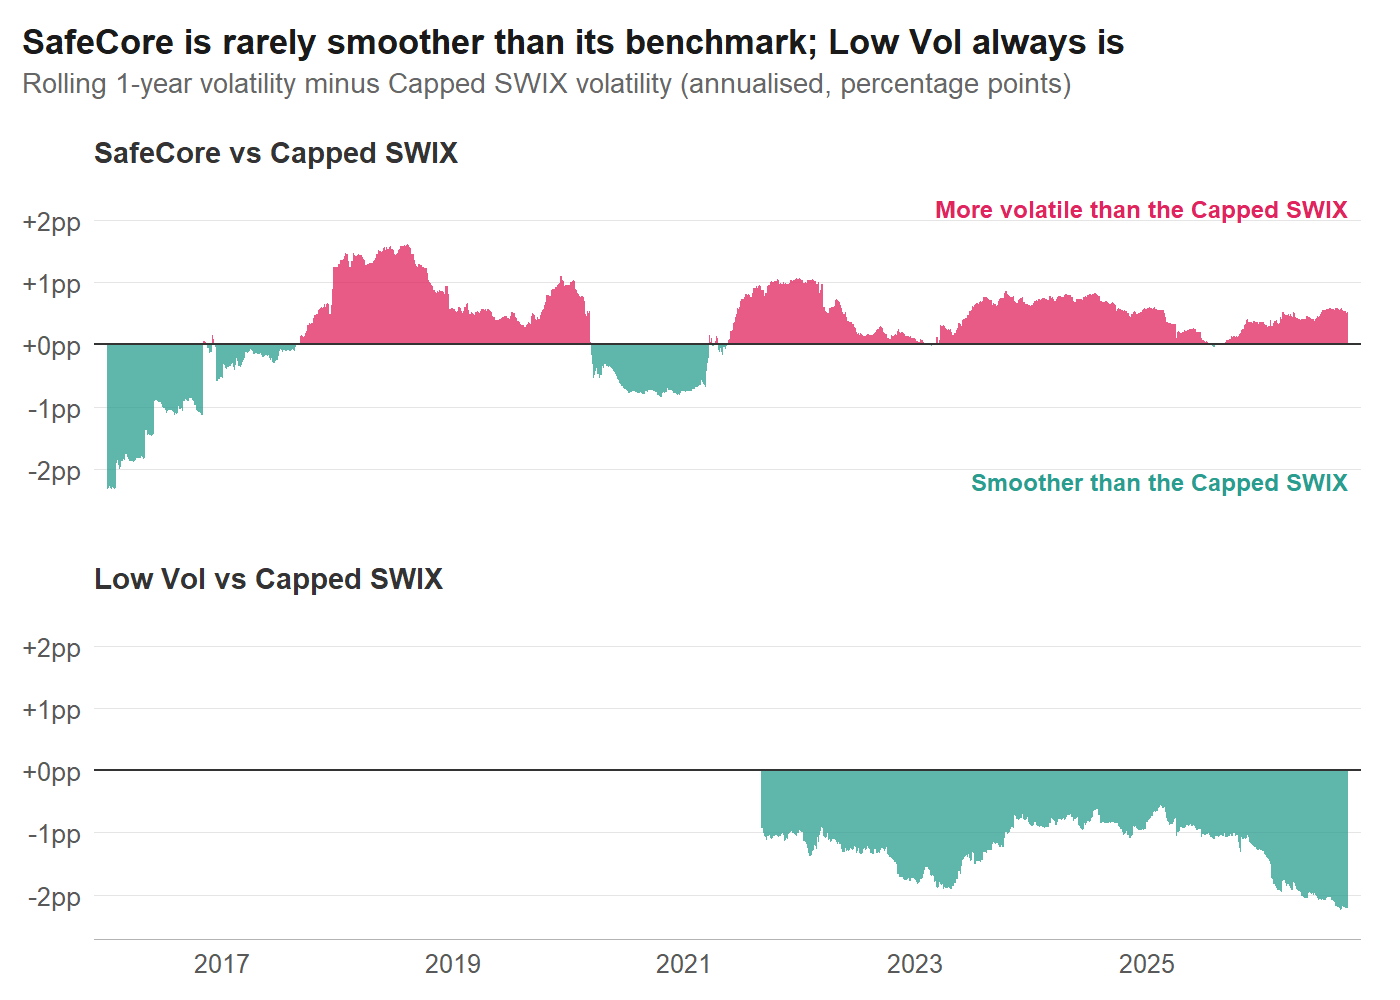
\includegraphics[width=1\linewidth]{Question1_files/figure-latex/volratio-1} 

}

\caption{Rolling 1-year volatility of SafeCore and the Low Vol index against the Capped SWIX \label{volratio}}\label{fig:volratio}
\end{figure}

Figure \ref{capture} shows how each fund participates in market moves.
SafeCore's yearly points cluster around (1, 1): in most years it simply
captures all of the market's upside and all of its downside, with only
2016 and 2017 in the ideal quadrant and 2019 and 2024 in the worst. The
Low Vol index sits in the bottom-left, capturing only 80-88\% of both up
and down moves: a genuine low-beta strategy reduces both sides
symmetrically rather than offering free downside protection.

\begin{figure}[H]

{\centering 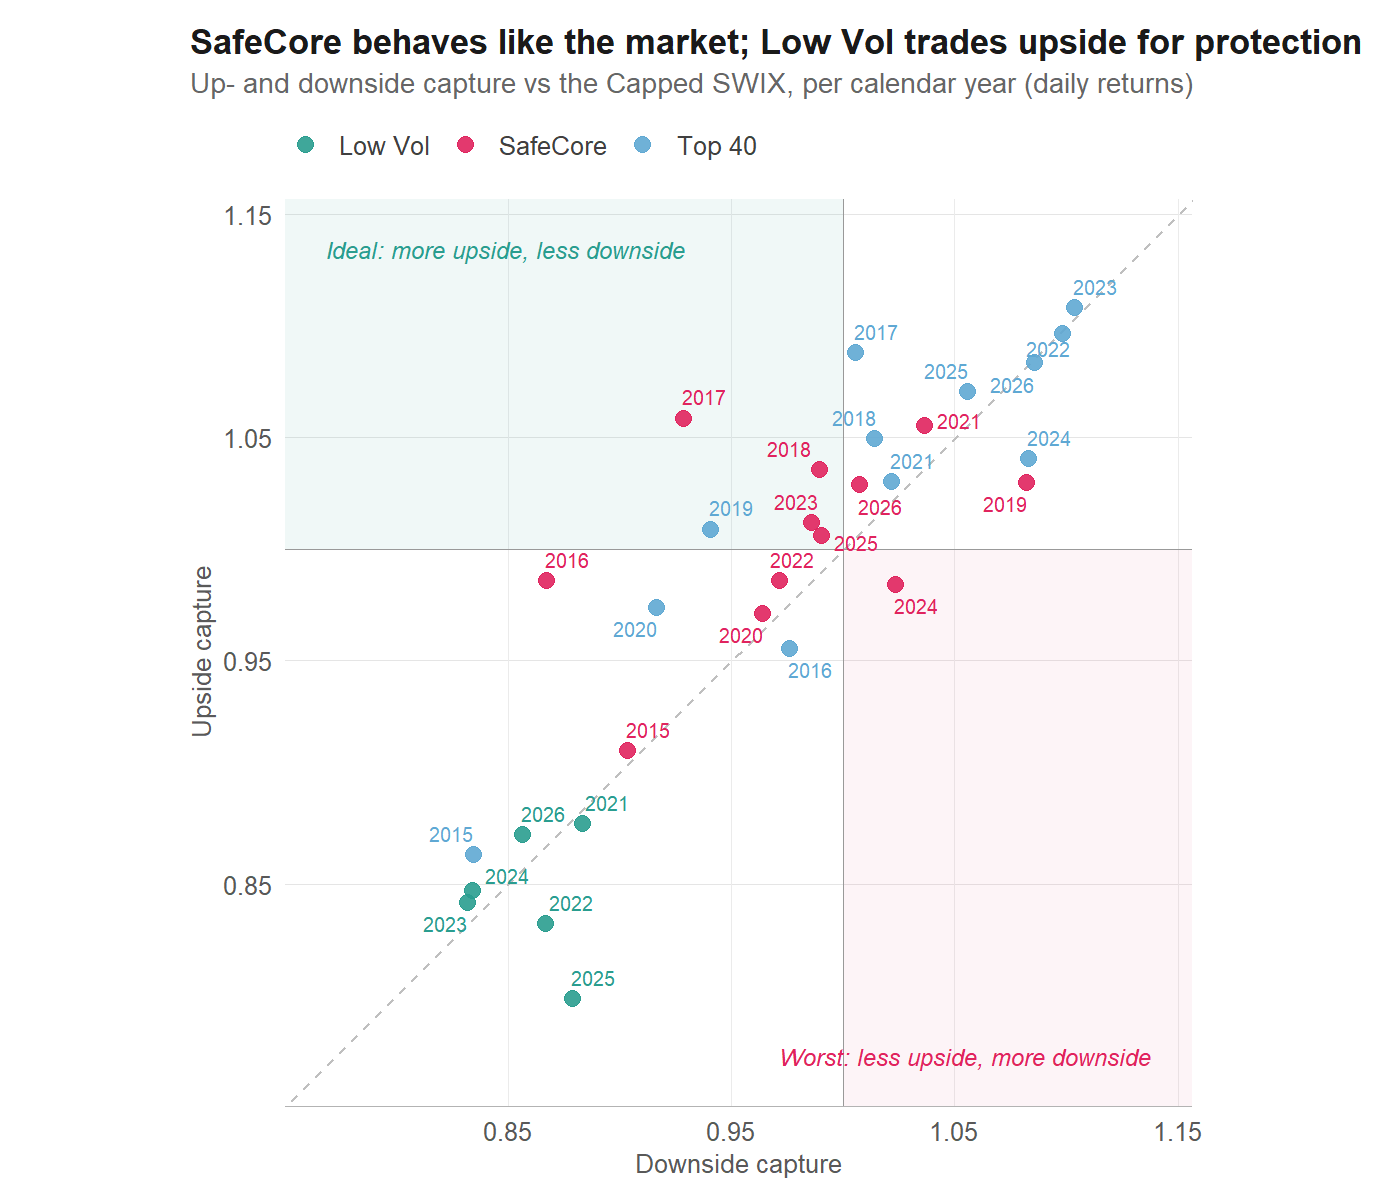
\includegraphics[width=1\linewidth]{Question1_files/figure-latex/capture-1} 

}

\caption{Up- and downside capture vs the Capped SWIX by calendar year \label{capture}}\label{fig:capture}
\end{figure}

The stress tests in Figure \ref{stress} and the regime analysis in
Figure \ref{regimes} confirm that SafeCore's edge is not protection. It
beat the benchmark in 7 of 10 stress episodes, but mostly by less than
1.5 percentage points, and it did worse in the most relevant episode for
the seminar's argument, the 2022 oil shock. Its excess return is similar
across calm, normal and stressed VIX regimes (about 0.2\% a month), and
it beats the benchmark in only half of stressed months: SafeCore's
outperformance is a steady stock-selection edge, not a
volatility-management one.

\begin{figure}[H]

{\centering 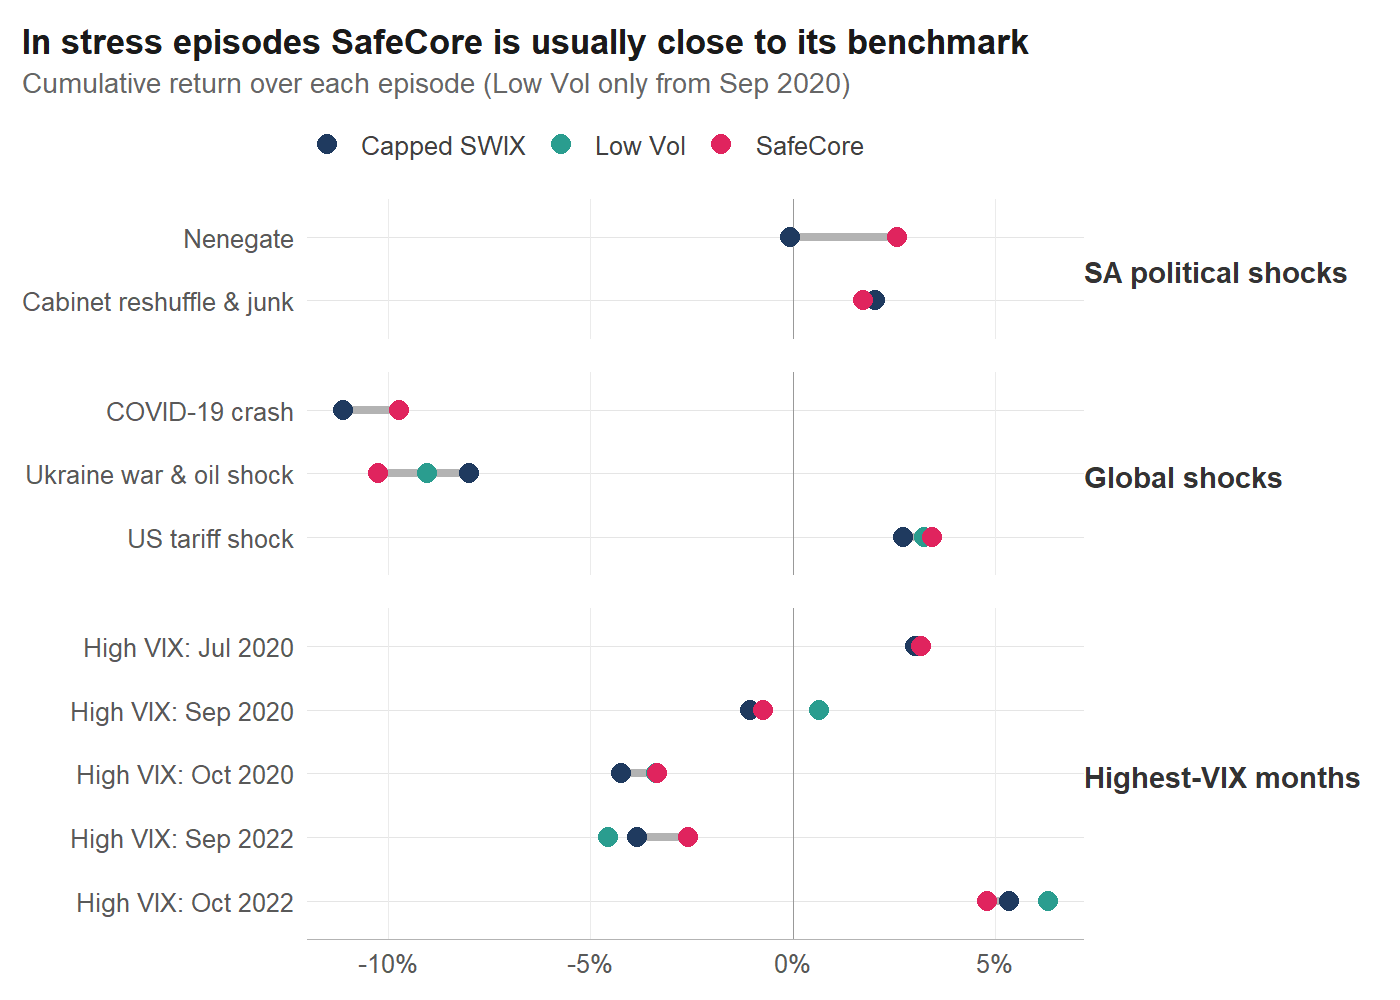
\includegraphics[width=1\linewidth]{Question1_files/figure-latex/stress-1} 

}

\caption{Cumulative returns in stress episodes \label{stress}}\label{fig:stress}
\end{figure}

\begin{figure}[H]

{\centering 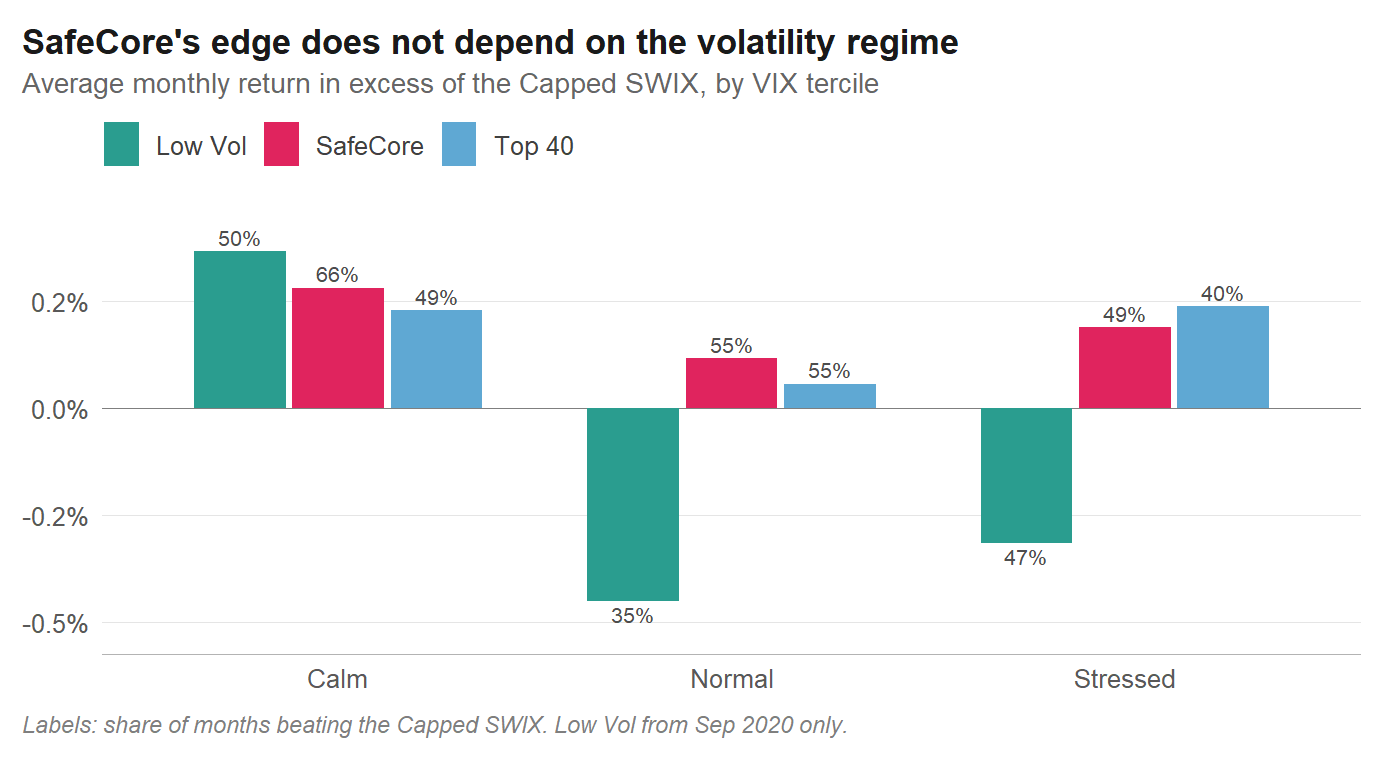
\includegraphics[width=1\linewidth]{Question1_files/figure-latex/regimes-1} 

}

\caption{Monthly excess return over the Capped SWIX by VIX regime \label{regimes}}\label{fig:regimes}
\end{figure}

\subsection{Sources of volatility}\label{sources-of-volatility}

A stock's share of a fund's risk can differ greatly from its weight,
because risk depends on its volatility and on how it co-moves with the
other holdings. SafeCore's variance is therefore decomposed into stock
and sector contributions each month (Euler risk contributions, using a
Ledoit-Wolf shrunk covariance matrix estimated over the previous year).
Figure \ref{sectorrisk} shows that resources have always been an
important source of risk, and this has become more prevalent recently:
in August 2026 they made up 40\% of the fund but 68\% of its risk
(Figure \ref{waffle}). Figure \ref{lollipop} identifies the culprits:
AngloGold Ashanti and Gold Fields together carry almost half of the
fund's risk, while banks and industrials (Standard Bank, Absa,
FirstRand, MTN, Naspers) contribute less risk than their weight and act
as diversifiers.

\begin{figure}[H]

{\centering 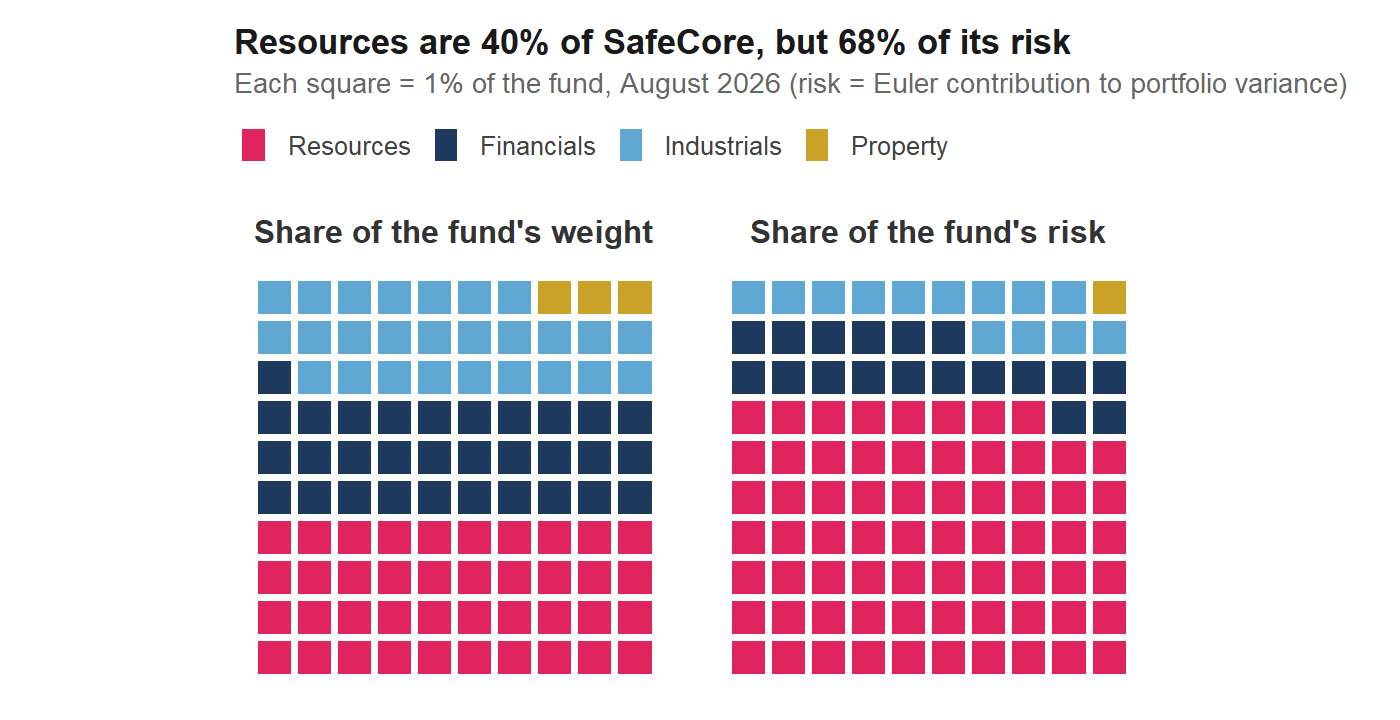
\includegraphics[width=1\linewidth]{Question1_files/figure-latex/waffle-1} 

}

\caption{Share of SafeCore's weight vs share of its risk by sector, latest month (each square = 1\%) \label{waffle}}\label{fig:waffle}
\end{figure}

\begin{figure}[H]

{\centering 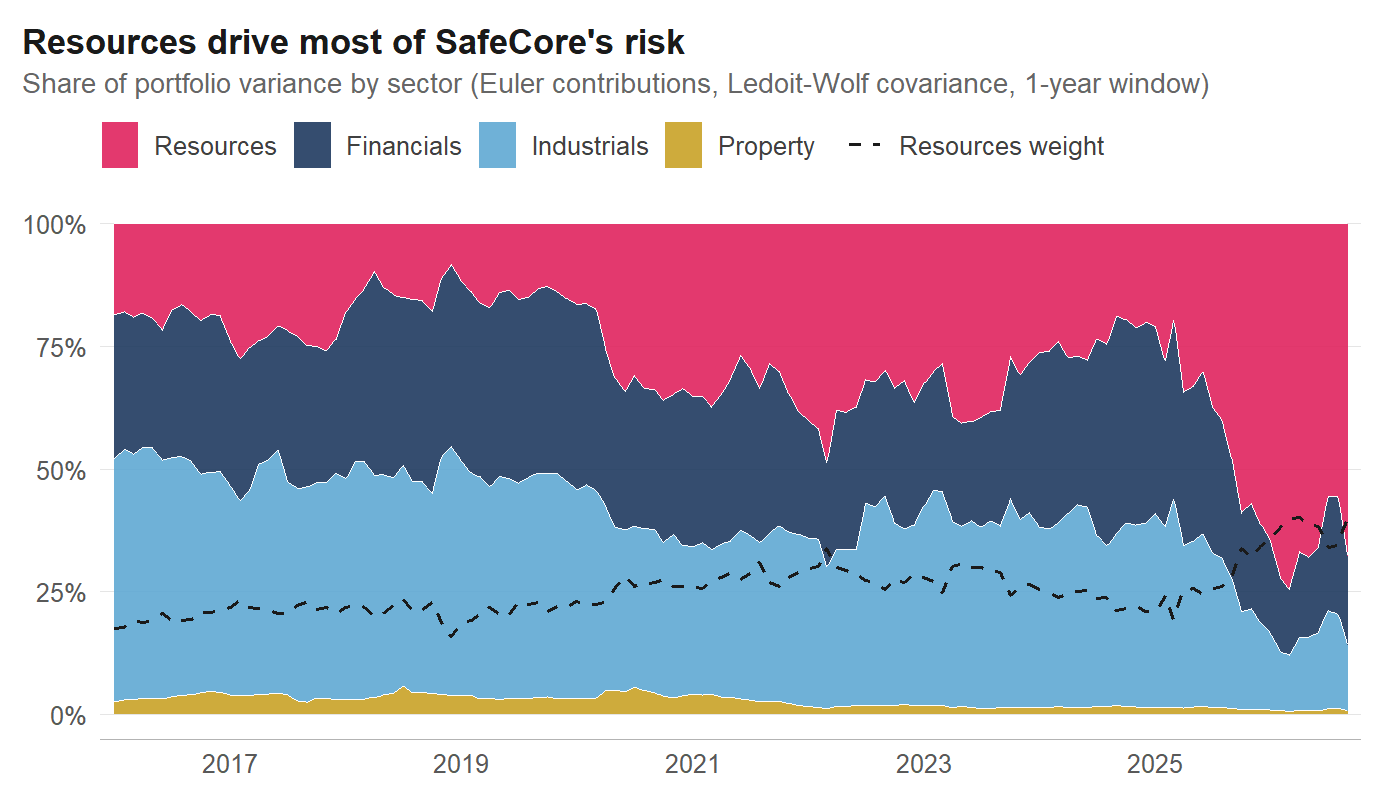
\includegraphics[width=1\linewidth]{Question1_files/figure-latex/sectorrisk-1} 

}

\caption{Sector contributions to SafeCore's risk \label{sectorrisk}}\label{fig:sectorrisk}
\end{figure}

\begin{figure}[H]

{\centering 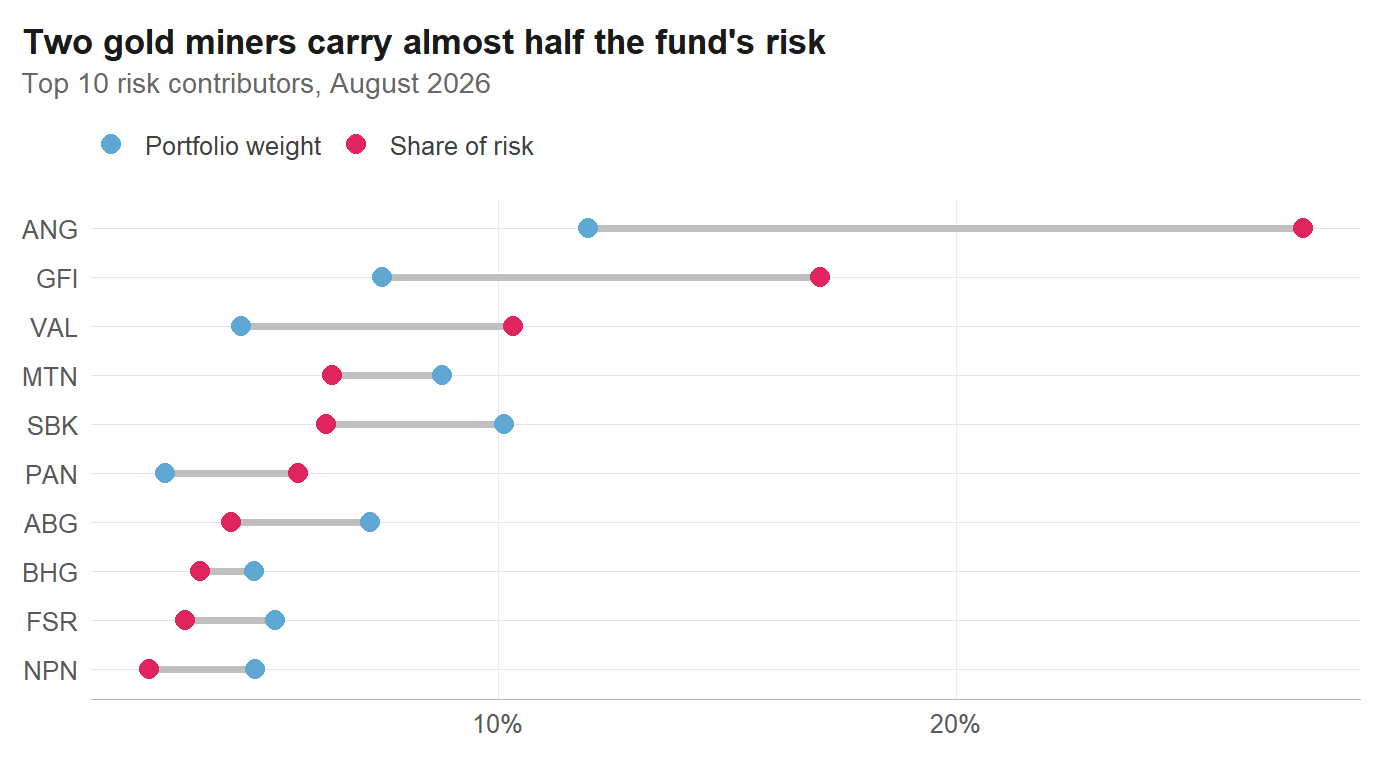
\includegraphics[width=1\linewidth]{Question1_files/figure-latex/lollipop-1} 

}

\caption{Weight vs share of risk, top 10 risk contributors \label{lollipop}}\label{fig:lollipop}
\end{figure}

Two structural features amplify this (Figure \ref{conchedge}). SafeCore
is concentrated: its effective number of stocks (17-22) is about half
that of the Capped SWIX, and it has fallen in 2026, so a few stocks can
dominate its risk. And it holds fewer pure rand hedges and rand-neutral
stocks than the benchmark, but more rand plays, alongside
currency-sensitive ``rand leverage'' miners. This is not a profile that
cushions a global risk-off shock, which Part A showed to be the main
source of local volatility.

\begin{figure}[H]

{\centering 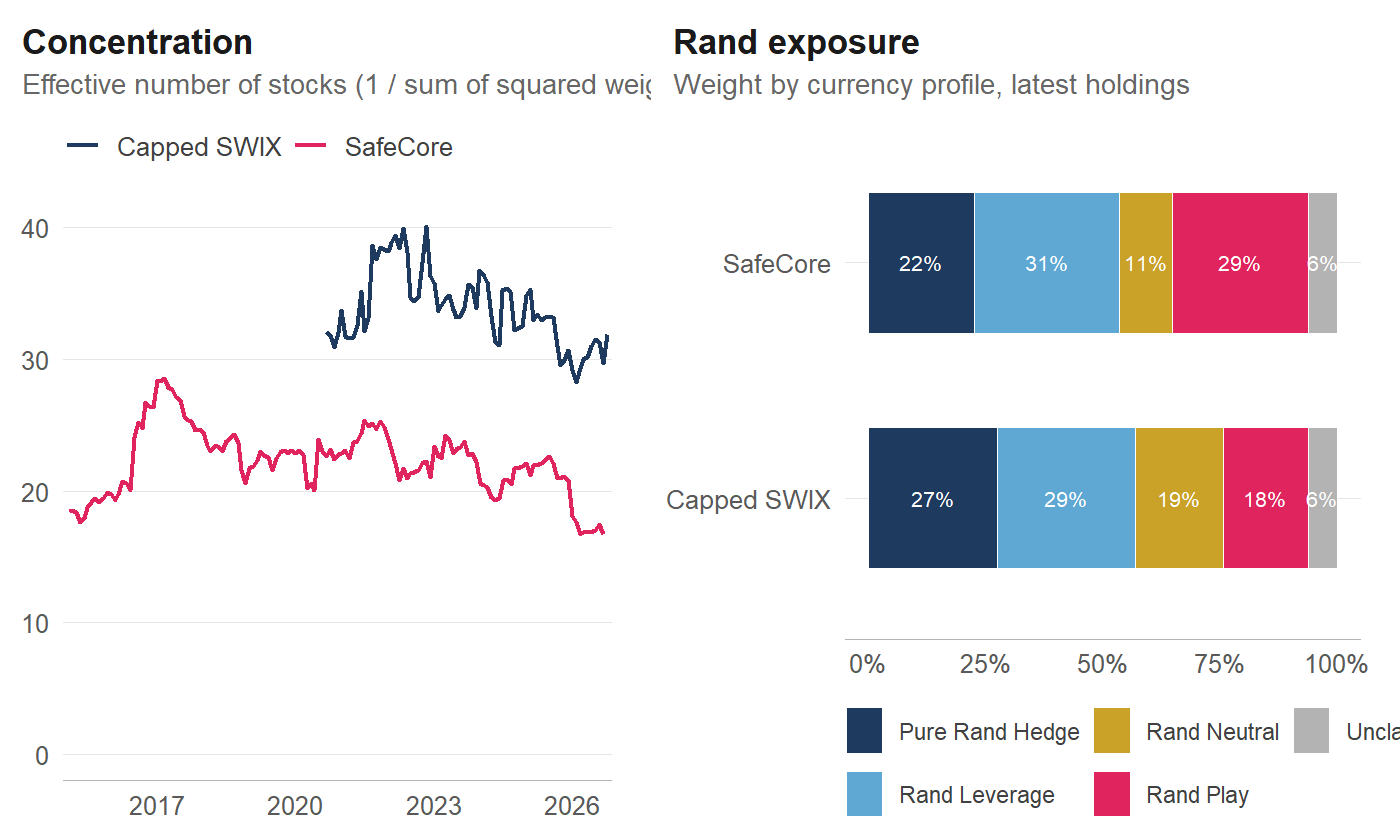
\includegraphics[width=1\linewidth]{Question1_files/figure-latex/conchedge-1} 

}

\caption{Concentration (left) and rand-hedge profile at the latest date (right) \label{conchedge}}\label{fig:conchedge}
\end{figure}

\subsection{Factor exposures}\label{factor-exposures}

Two scores are constructed from price data at each month-end. Momentum
is the return from six months to one month ago (skipping the latest
month, whose short-term reversals would add noise), and low volatility
is minus the stock's six-month realised volatility, so that a high score
means a low-volatility stock. Both are standardised across stocks each
month and capped at \(\pm 3\) to limit the influence of illiquid stocks
with extreme moves.

Figure \ref{scores} compares them with the third party's scores. The own
momentum score agrees well with the vendor's (an average rank
correlation of about 0.6); the largest disagreements are the gold and
platinum miners, which the vendor still rates as high-momentum,
suggesting it uses a longer look-back. The own low-volatility score, by
contrast, is essentially unrelated to the vendor's ``Volatility
Sensitivity'' (rank correlation of about 0.1), and further checks show
the vendor measure is also barely related to realised volatility or
market beta. It appears to capture sensitivity to \emph{changes} in
market volatility rather than the level of volatility, so it should not
be read as a low-volatility score.

\begin{figure}[H]

{\centering 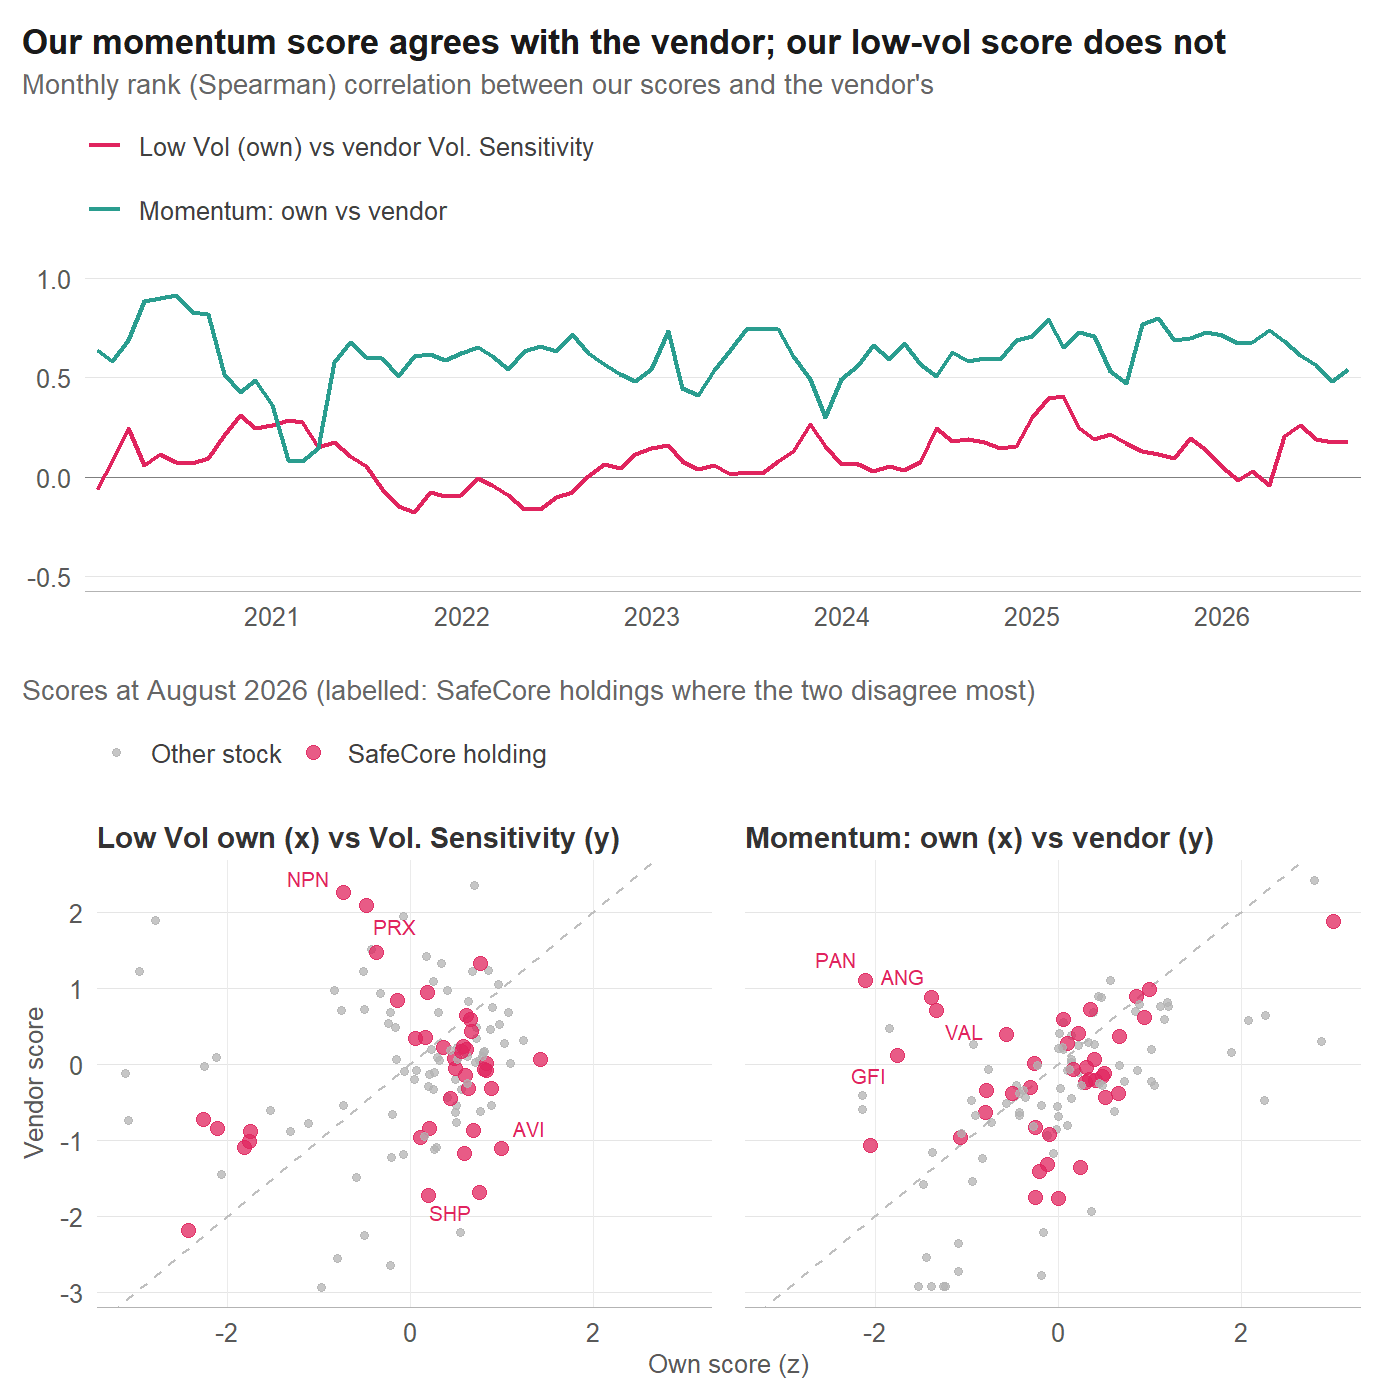
\includegraphics[width=1\linewidth]{Question1_files/figure-latex/scores-1} 

}

\caption{Own vs third-party factor scores \label{scores}}\label{fig:scores}
\end{figure}

To contextualise SafeCore, the stock scores are aggregated into
composite portfolio scores (weighted averages over each portfolio's
holdings) for SafeCore and the Value, Momentum, Quality and Low Vol
indexes. Because the vendor's scores turn out to be benchmark-relative
(the Capped SWIX scores almost exactly zero on every vendor factor), all
exposures are expressed relative to the Capped SWIX. The factor indexes
line up with their labels, which validates the approach. Against them,
SafeCore's fingerprint (Figure \ref{finger}), whose shape is closest to
the Momentum and Quality indexes and furthest from Low Vol, is that of a
quality-momentum fund with a mild value tilt and no low-volatility tilt
at all. Figure \ref{drift} adds the timing: SafeCore's momentum exposure
rose sharply in 2026 while its low-volatility exposure turned negative,
which is how the fund drifted into the volatile gold miners that now
dominate its risk.

\begin{figure}[H]

{\centering 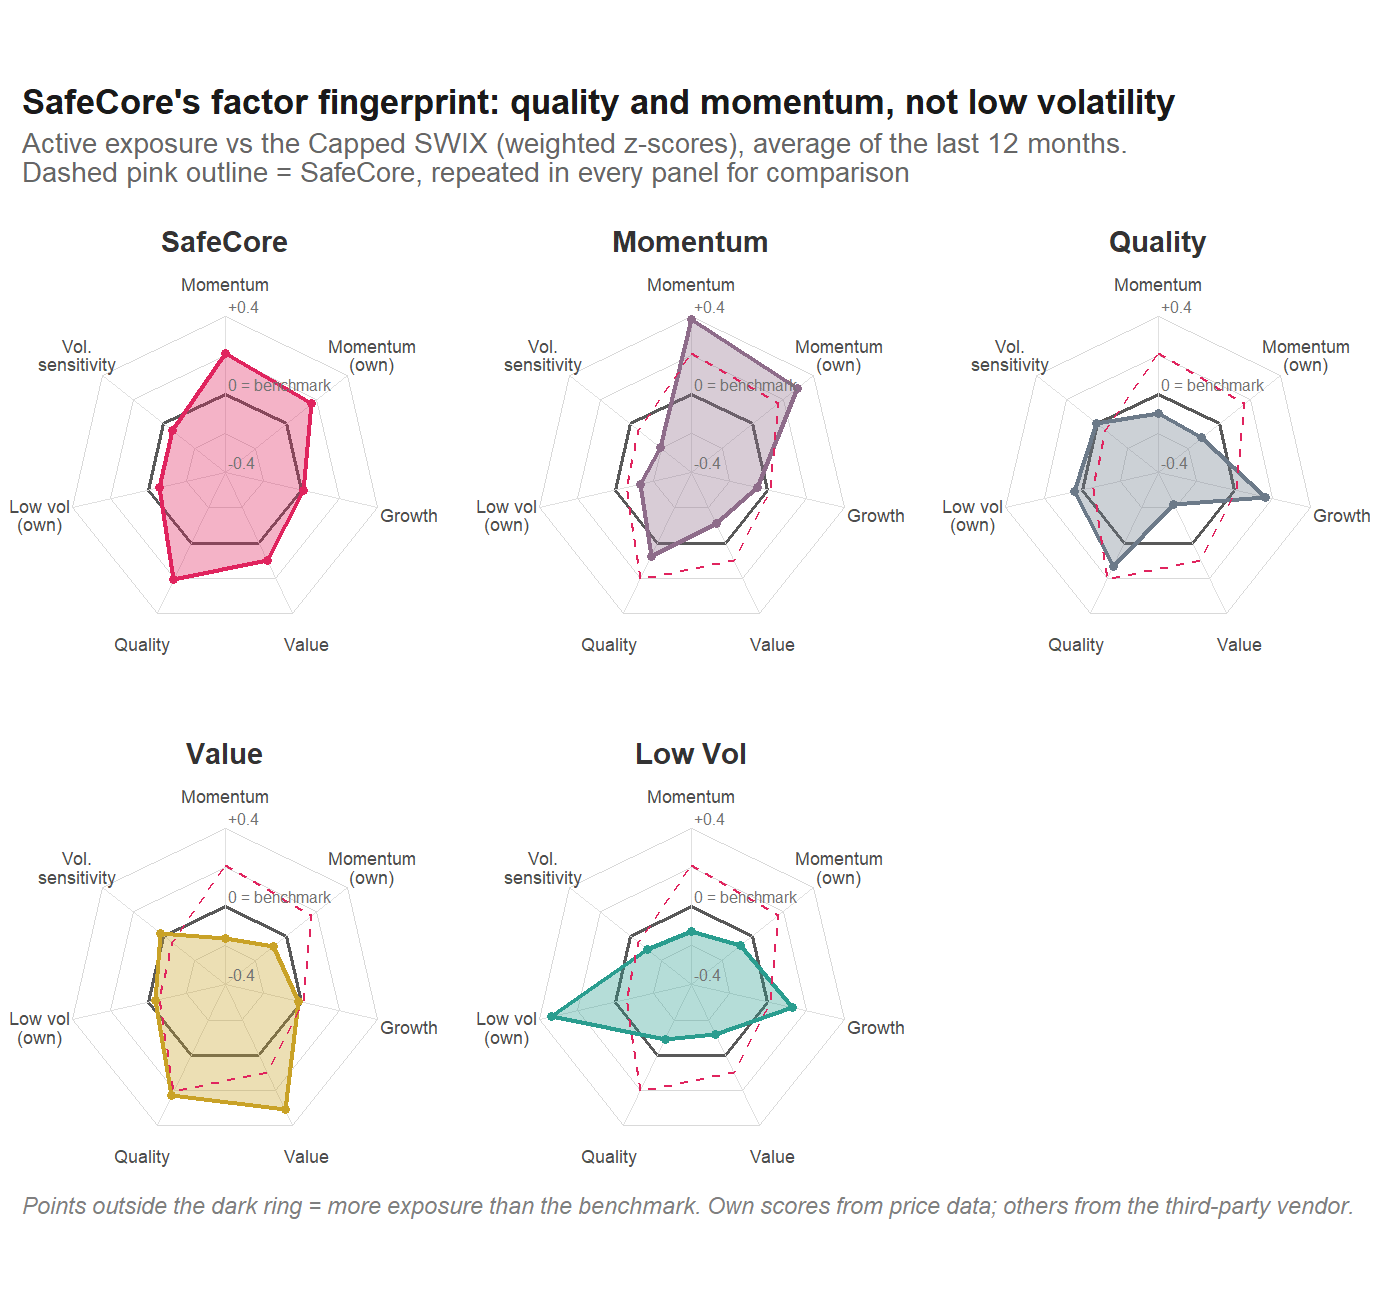
\includegraphics[width=1\linewidth]{Question1_files/figure-latex/finger-1} 

}

\caption{Factor fingerprints: active exposures vs the Capped SWIX, last 12 months (dashed outline = SafeCore) \label{finger}}\label{fig:finger}
\end{figure}

\begin{figure}[H]

{\centering 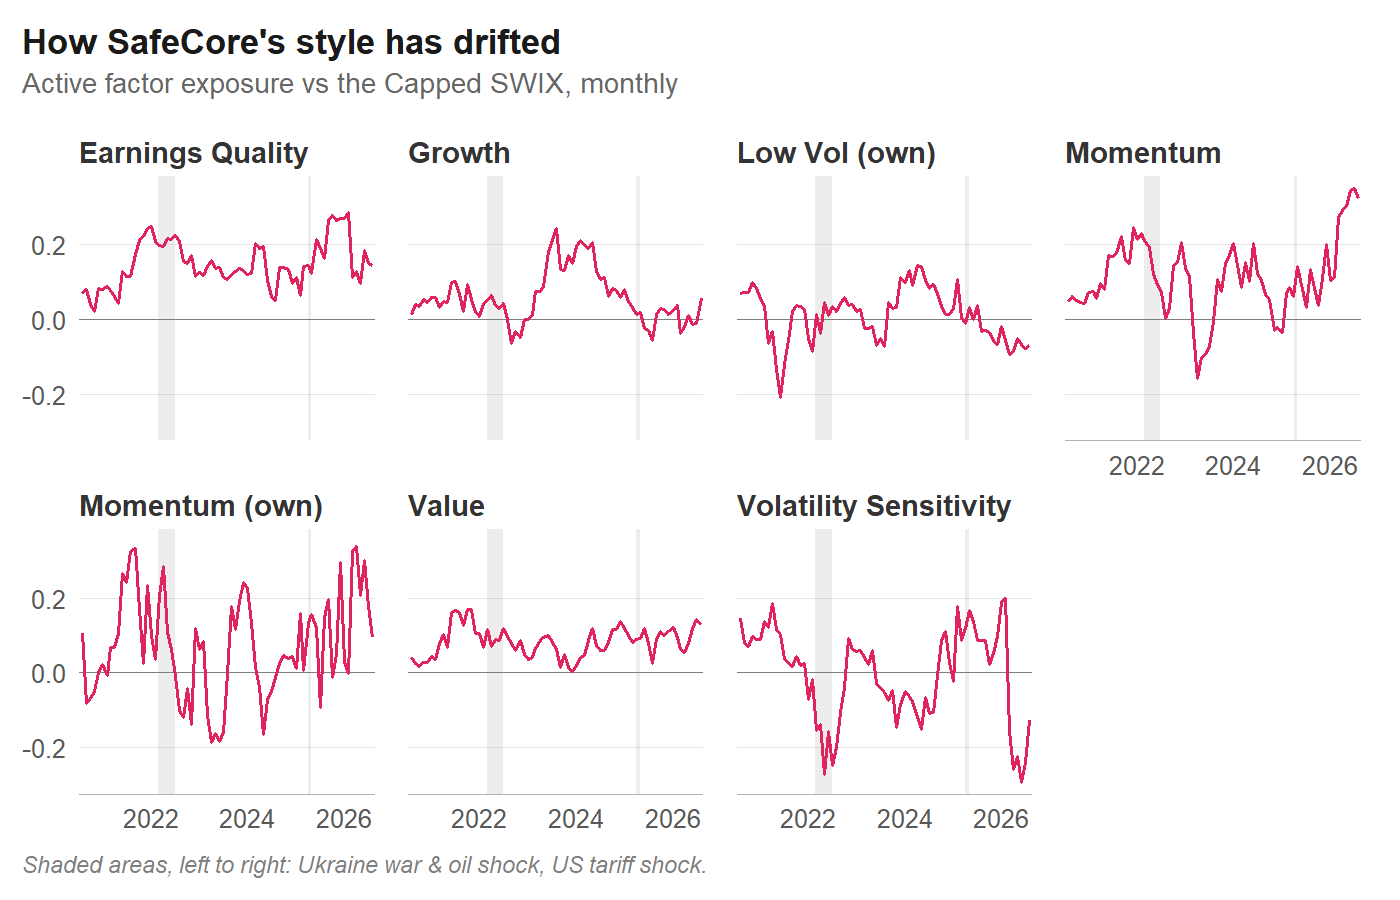
\includegraphics[width=1\linewidth]{Question1_files/figure-latex/drift-1} 

}

\caption{SafeCore's active factor exposures over time \label{drift}}\label{fig:drift}
\end{figure}

\subsection{Implications for Part B}\label{implications-for-part-b}

SafeCore has been a good fund, but not a risk ballast. It outperformed
its benchmark by close to 3\% a year, yet with the same volatility,
near-full participation in market falls and no consistent advantage in
stressed periods. Its volatility is concentrated in a handful of
resource stocks, its effective breadth is half the benchmark's, and its
momentum tilt has recently pulled it further into these names. If the
team wants SafeCore to offer some protection in the global risk-off
episodes identified in Part A, practical steps would be to budget risk
rather than only weights (capping single-stock and sector risk
contributions), to monitor the momentum tilt for crowding into one
theme, and to add an explicit low-volatility tilt or sleeve, accepting,
as the Low Vol index shows, that this costs some upside in strong
markets.

\section{\texorpdfstring{Part C: The alpha opportunity since 2020
\label{PartC}}{Part C: The alpha opportunity since 2020 }}\label{part-c-the-alpha-opportunity-since-2020}

Active managers often add value when stocks behave differently from one
another. The alpha opportunity is therefore measured from two
complementary angles: dispersion (how far apart stock returns are on a
given day) and correlation (how much stocks move together over time).
High dispersion with low correlation describes a stock-picker's market;
low dispersion with high correlation a macro-driven one. Constituent
data is available from August 2020.

\subsection{Dispersion}\label{dispersion}

Dispersion is measured as the daily cross-sectional volatility (CSV) of
the Capped SWIX constituents, weighted by their previous-day index
weights: \[CSV_t = \sqrt{\sum_i w_{i,t-1}(R_{i,t} - \bar{R}_t)^2}\]
where \(\bar{R}_t\) is the weighted average (index) return. The weighted
measure is preferred because it reflects the opportunity relevant to a
fund benchmarked against the Capped SWIX, where a large move in a stock
with a negligible index weight matters little, and because the
unweighted measure is dominated by small, illiquid stocks with erratic
prices. Two corporate-action artefacts were removed before the
calculation (the listing of Richemont's shareholder warrants in November
2020, which shows a one-day ``return'' of over 369,000\%, and the
Fortress A/B share restructure in February 2024); the warrant print
alone would otherwise have tripled November 2020's dispersion.

Figure \ref{csv} shows that dispersion was high in late 2020, fell to
its lowest level in 2024 (an average daily CSV of about 1.6\%) and has
risen again to about 2.0\% in 2026. The unweighted measure follows the
same pattern at a higher level. Figure \ref{decomp} splits the weighted
variance exactly into a within-sector part (the stock-picking
opportunity) and a between-sector part (the sector-allocation
opportunity). Until 2024 about 80\% of dispersion came from within
sectors; since 2025 the between-sector share has risen sharply, to about
a third on average in 2026 and half in some months. This mirrors Part B:
resources, and gold miners in particular, have moved very differently
from the rest of the market, so sector calls now matter as much as stock
selection.

\begin{figure}[H]

{\centering 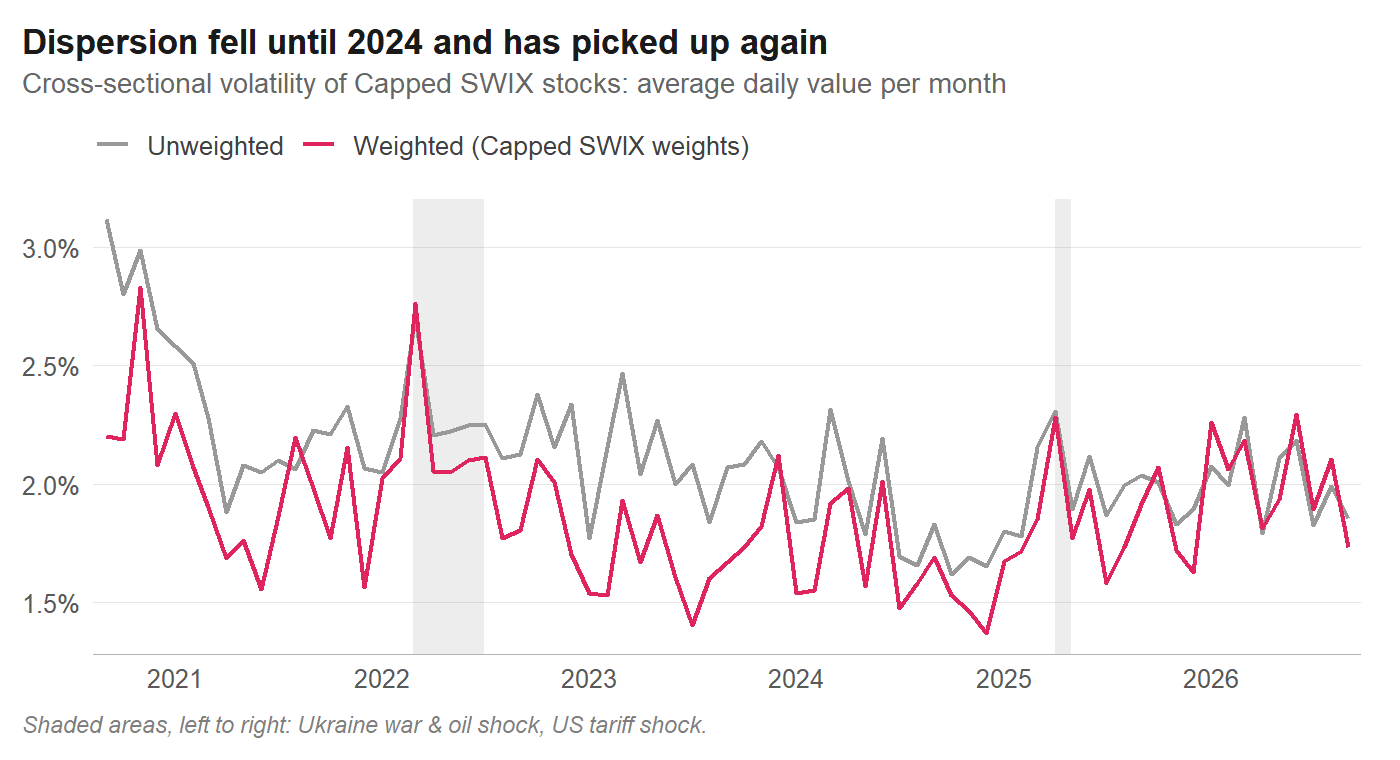
\includegraphics[width=1\linewidth]{Question1_files/figure-latex/csv-1} 

}

\caption{Cross-sectional volatility of Capped SWIX constituents \label{csv}}\label{fig:csv}
\end{figure}

\begin{figure}[H]

{\centering 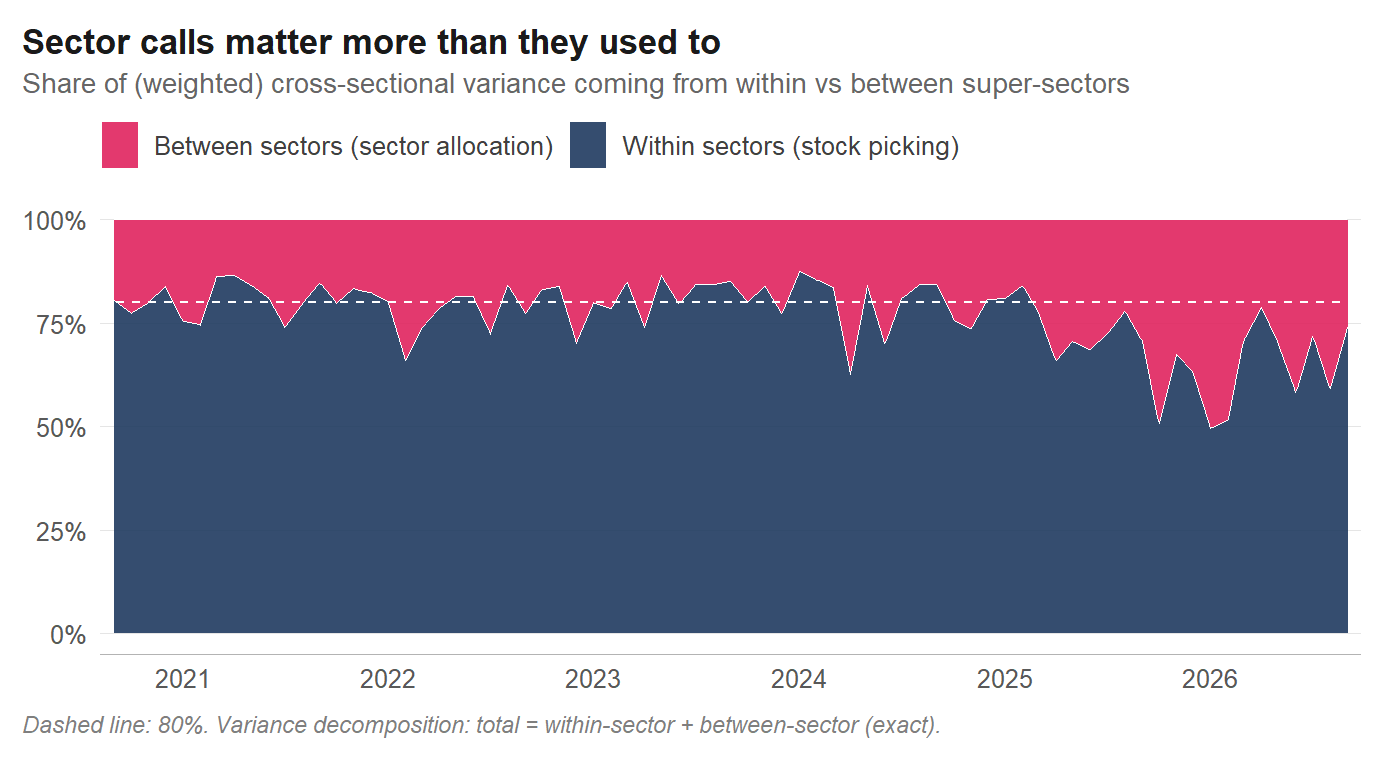
\includegraphics[width=1\linewidth]{Question1_files/figure-latex/decomp-1} 

}

\caption{Within- vs between-sector share of dispersion \label{decomp}}\label{fig:decomp}
\end{figure}

\subsection{Correlation}\label{correlation}

Figure \ref{paircor} shows the distribution of pairwise correlations
between Large Cap stocks over rolling 63-day windows. Showing the median
and the middle 50\% of pairs, rather than a single average, reveals
whether all stocks were moving together or only some. Correlations
peaked in 2022, the year of the Ukraine war and aggressive rate hikes,
when the whole distribution shifted upwards, and fell to their lowest
levels in 2024-2025, when stocks traded more on their own fundamentals.

\begin{figure}[H]

{\centering 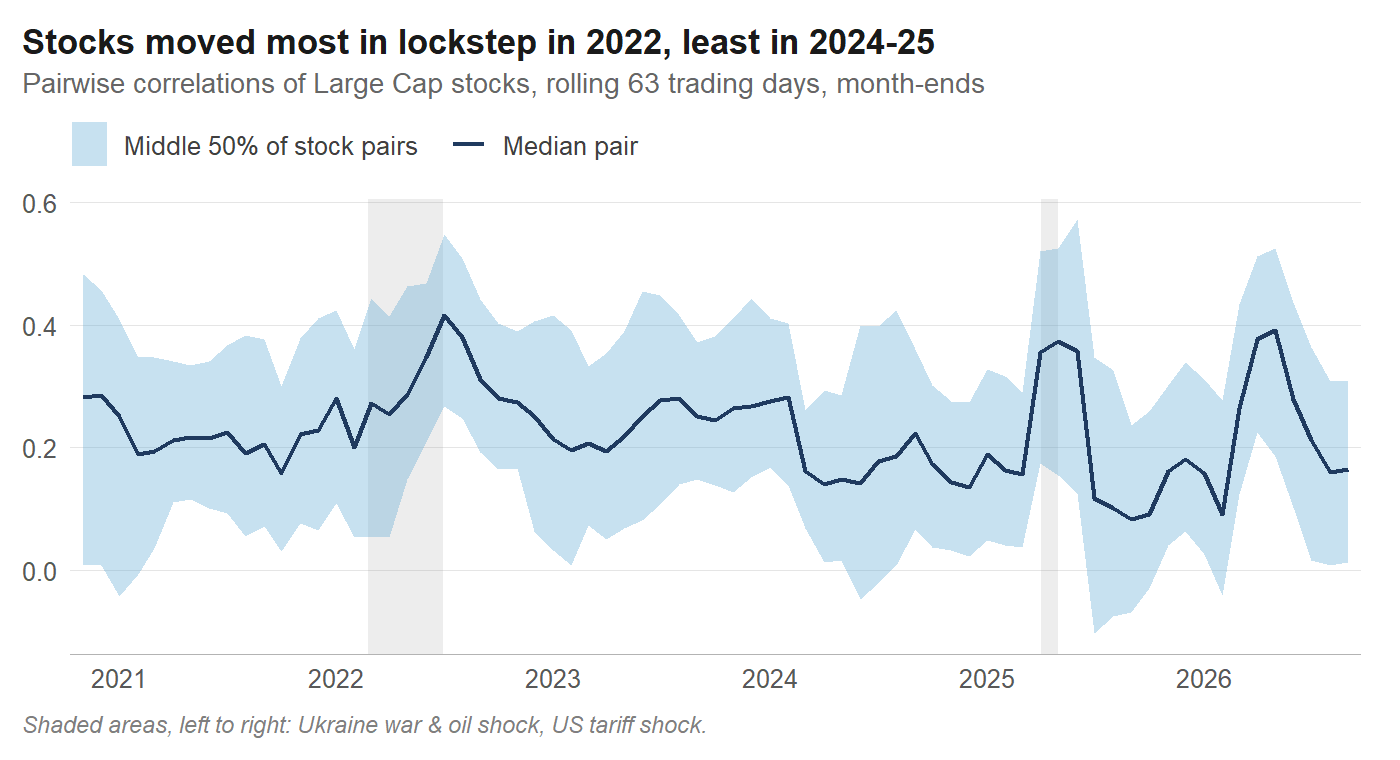
\includegraphics[width=1\linewidth]{Question1_files/figure-latex/paircor-1} 

}

\caption{Rolling pairwise correlations of Large Cap stocks \label{paircor}}\label{fig:paircor}
\end{figure}

\subsection{Mapping the alpha
opportunity}\label{mapping-the-alpha-opportunity}

Dispersion and correlation are only weakly related in this sample (a
correlation of 0.17), so they capture different aspects of the
opportunity. Figure \ref{quad} plots them against each other: 2022 sits
in the macro-driven half of the map, 2023-2024 in the low-dispersion
half, and many months of 2025-2026 in the stock-picker's quadrant. The
map is summarised with an Alpha Opportunity Index, equal to standardised
dispersion minus standardised correlation (Figure \ref{oppindex}). The
opportunity was strong in late 2020 and early 2022, weak from mid-2022
to 2024, and has improved markedly since 2025.

\begin{figure}[H]

{\centering 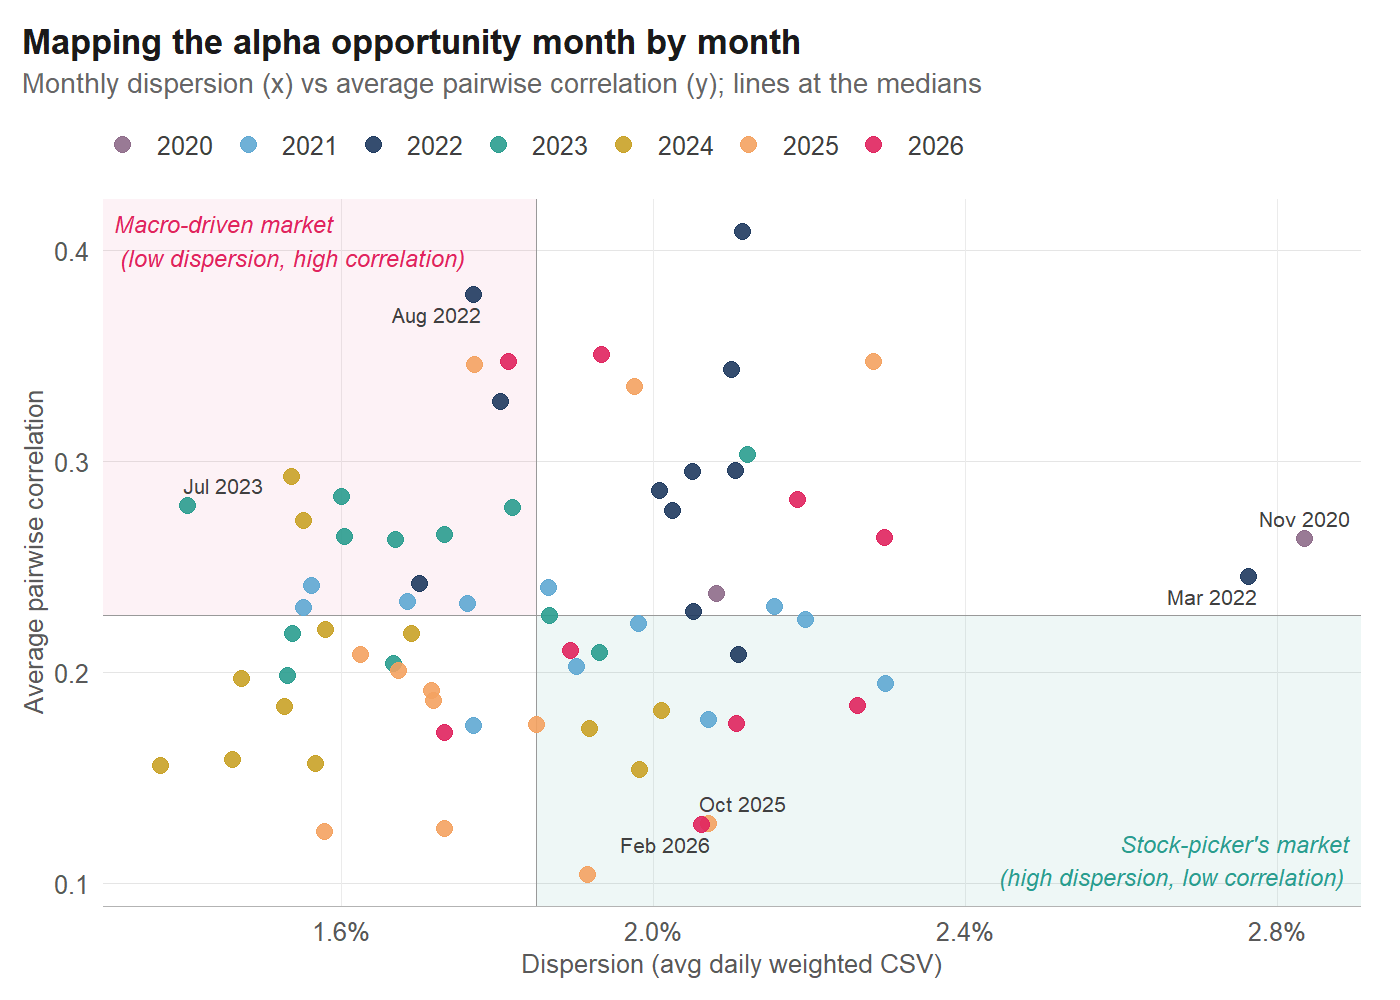
\includegraphics[width=1\linewidth]{Question1_files/figure-latex/quad-1} 

}

\caption{Monthly dispersion vs average pairwise correlation \label{quad}}\label{fig:quad}
\end{figure}

\begin{figure}[H]

{\centering 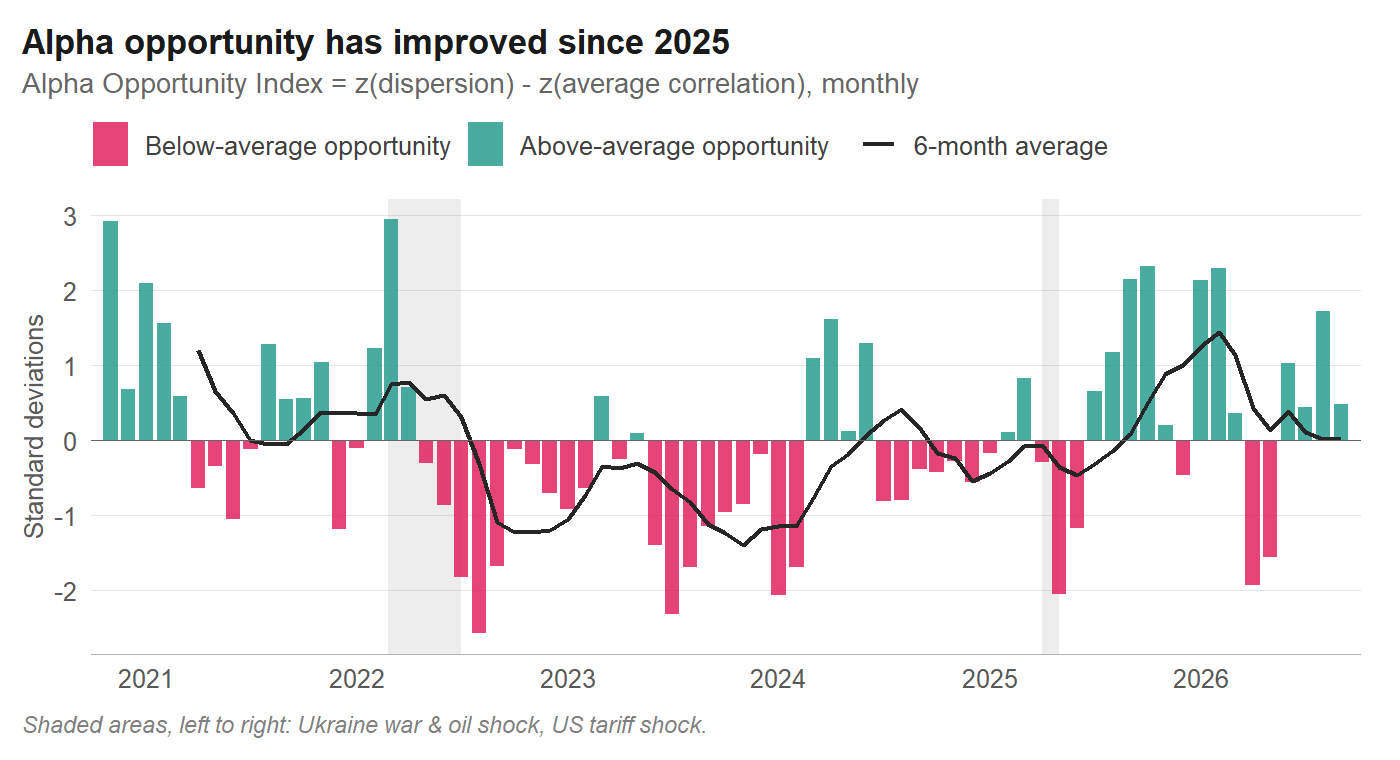
\includegraphics[width=1\linewidth]{Question1_files/figure-latex/oppindex-1} 

}

\caption{Alpha Opportunity Index \label{oppindex}}\label{fig:oppindex}
\end{figure}

To check that the index reflects a real opportunity, Figure
\ref{realised} compares it with two payoffs available in the data: the
return gap between the best and worst quintile of Capped SWIX stocks
each month, and the gap between the best and worst factor index. In
high-opportunity months the stock-quintile spread averaged 26\% a month,
against 22\% in low-opportunity months (a correlation of 0.51 with the
index), whereas the factor spread is small and only weakly related. The
index therefore captures a genuine stock-selection opportunity, though
it says little about style timing.

\begin{figure}[H]

{\centering 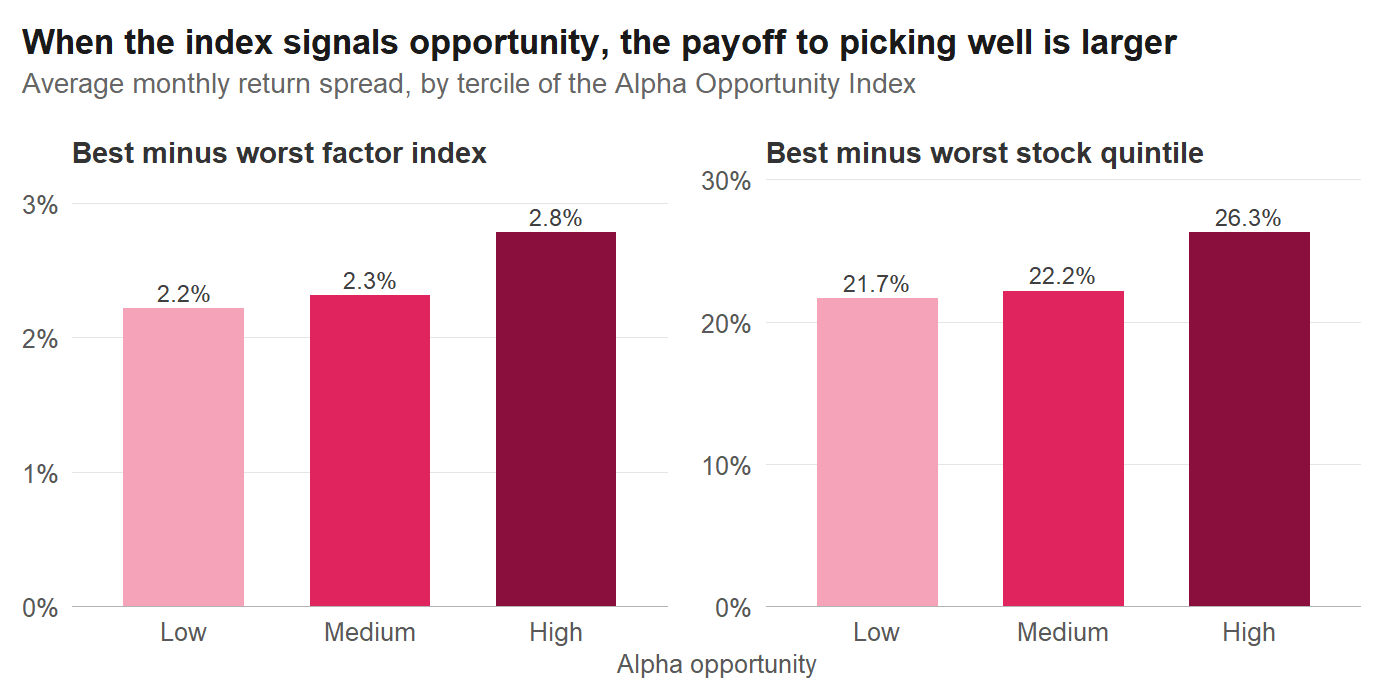
\includegraphics[width=1\linewidth]{Question1_files/figure-latex/realised-1} 

}

\caption{Return spreads by level of the Alpha Opportunity Index \label{realised}}\label{fig:realised}
\end{figure}

\subsection{Alpha opportunity and global macro
factors}\label{alpha-opportunity-and-global-macro-factors}

Figures \ref{leadlag} and \ref{macroreg} relate dispersion, correlation
and the opportunity index to the global macro measures from Part A.
Higher equity fear (VIX, VXEEM) raises dispersion, but it also raises
correlation, and predicts higher correlation the following month, so its
net effect on the opportunity is small: prices spread out, but
increasingly in response to the same risk-on/risk-off swings. Bond and
currency volatility are what hurt stock pickers. High US bond volatility
(MOVE) goes with lower dispersion and higher correlation and has the
strongest negative relationship with the opportunity index; global FX
and rand volatility show the same pattern. These measures are also more
strongly related to \emph{next} month's opportunity than to this
month's, so rising rate and currency volatility act as an early warning
of a more correlated, less rewarding market, as in 2022. Policy
uncertainty (EPU) again shows little relationship, consistent with Part
A.

\begin{figure}[H]

{\centering 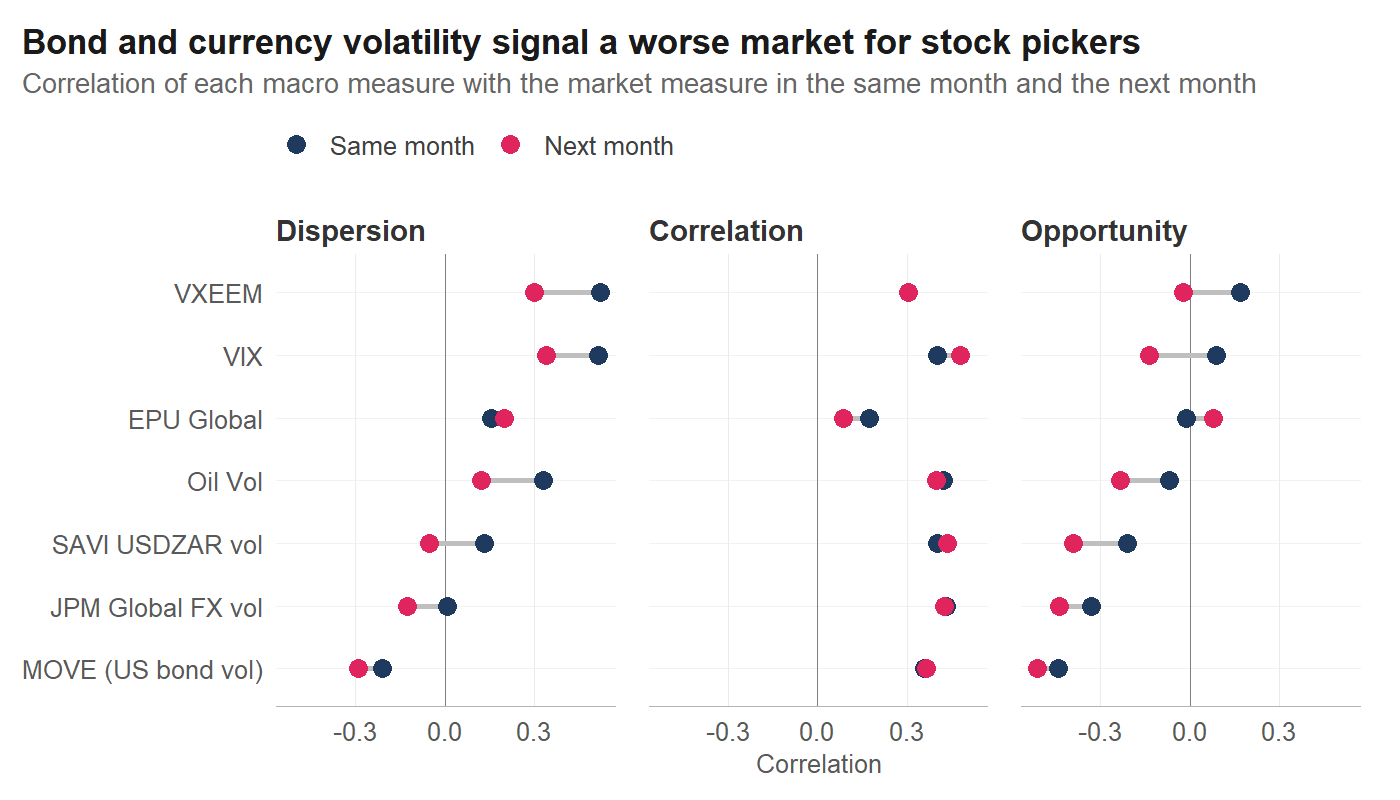
\includegraphics[width=1\linewidth]{Question1_files/figure-latex/leadlag-1} 

}

\caption{Same-month and next-month correlation of macro measures with dispersion, correlation and the opportunity index \label{leadlag}}\label{fig:leadlag}
\end{figure}

\begin{figure}[H]

{\centering 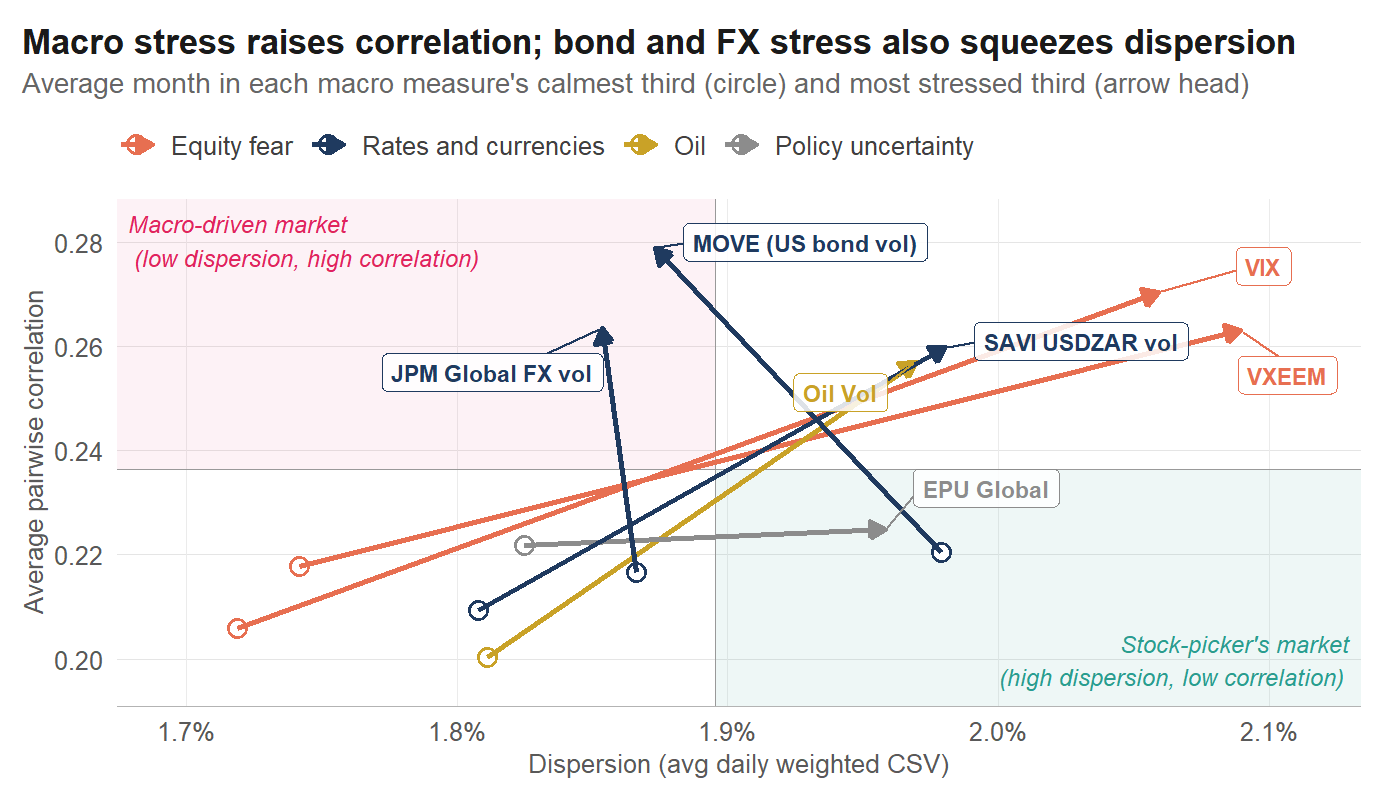
\includegraphics[width=1\linewidth]{Question1_files/figure-latex/macroreg-1} 

}

\caption{Dispersion and correlation in low vs high macro regimes \label{macroreg}}\label{fig:macroreg}
\end{figure}

These macro relationships are correlations estimated on about six years
of monthly data and are sensitive to a few episodes (2022 in
particular), so they should be read as indicative rather than causal.
The quintile spread is also a foresight measure: it shows how much there
was to gain from stock selection, not what any manager actually earned.

\section{\texorpdfstring{Conclusion
\label{Conclusion}}{Conclusion }}\label{conclusion}

The three parts give a consistent picture. Local volatility has not
moved to a permanently higher level, but volatility episodes have become
more frequent and are largely imported, through global risk-off shocks
and oil price volatility. SafeCore has added return but has not
protected investors in those episodes: its risk is concentrated in a few
resource stocks and its quality-momentum style has no low-volatility
tilt. Meanwhile, the opportunity to add value through stock selection
has improved since 2025, although more of it now comes from sectors
moving apart, and rising bond and currency volatility have tended to
signal tougher conditions for stock pickers. The implication for the
team is that SafeCore can keep its stock-selection edge while building
in a risk ballast aimed at the shocks that actually drive local
volatility: limiting single-stock and sector risk, adding a
low-volatility tilt, and monitoring global rate and currency volatility
as early warnings.

\bibliography{Tex/ref}





\end{document}
